% This document provides the style to be used for a MSc Thesis at the
% Parallel and Distributed Systems group
\documentclass[11pt,twoside,a4paper,openright]{report}

% math packages
\usepackage{amsmath}
\usepackage{amssymb}

% textblocks for title page
\usepackage[absolute]{textpos}

% use babel for proper hyphenation
\usepackage[british]{babel}

% Graphics: different for pdflatex or dvi output, choose one
%%\usepackage[dvips]{graphicx}
\usepackage[pdftex]{graphicx}
\usepackage{graphicx}

\usepackage{epstopdf}
\usepackage{rotating}
\usepackage{subcaption}

% FONT
\usepackage[scaled=.92]{helvet}
%\usepackage{times}
\usepackage{textcomp}
\usepackage{eurosym}

% for url's use "\url{http://www.google.com/}"
\usepackage{url}
\usepackage[plainpages=false]{hyperref} 

% Table
\usepackage{threeparttable, tablefootnote}
\usepackage{tabularx}
\usepackage{multirow}

% References
\usepackage{flushend}

% Tikz
\usepackage{tikz}
\usepackage{circuitikz}


% Information that will be filled in at various points in the report
\newcommand{\reportTitle}{Transiently-powered Battery-free Robot}
\newcommand{\reportAuthor}{Koen Schaper}
\newcommand{\reportEmail}{kpschaper@gmail.com}
\newcommand{\reportUrlEmail}{\href{mailto:\reportEmail}{\reportEmail}}
\newcommand{\reportMSC}{Embedded Systems} %{Embedded Systems}{Computer Engineering}{Computer Science}{Electrical Engineering}
\newcommand{\reportDate}{\today} %TODO: Dit is de datum van uitgifte van final versie aan de afstudeer commissie 
\newcommand{\presentationDate}{15 December 2017}
\newcommand{\graduationCommittee}{
prof. dr. K.G. Langendoen (chair) & Delft University of Technology \\
dr. Przemys\l{}aw Pawe\l{}czak (supervisor) & Delft University of Technology \\
dr. Javier Alonso-Mora & Delft University of Technology \\
} % The order of listing the names: Graduation prof, supervisor(s), others ordered by title + alphabetical 
%examples: 
%prof. dr. ir. H. J. Sips (chair) & Delft University of Technology \\ 
%ir. dr. D. H. J. Epema           & Delft University of Technology \\ 
\newcommand{\reportAbstract}{
	%Small robotic platforms have become increasingly popular as an educational toy for kids and are widely used by researchers to study swarm behavior with a collective of robots.
	Collectives of miniature robots are envisioned to have future applications in for example surveillance, search and rescue, and exploration. 
	However, before these robots can become applicable in real world applications, a fundamental challenge related to supply of energy needs to be addressed first.
	The operation time of small robots is currently limited by the energy storage in batteries.
	New advancements in batteries are not expected to happen anytime soon, as history shows that new battery technologies are slow emerging.
	This thesis proposes to replace the battery with an energy harvester and temporarily store harvested energy in a supercapacitor.
	This results in a new phenomenon to be taken into consideration: frequent power failures due to the the intermittent availablility of energy.
	Intermittency is currently not taken into account in the development process of a robot, and its effect on control techniques and locomotion is, therefore, unexplored.
	In this work a transiently-powered battery-free robot is developed that purely operates from harvested energy from light.
	The robot is able to move with a 16\% power duty cycle, using a lighting setup consisting of four halogen lamps.
	With the help of local feedback the robot is able to perform controlled movements, while peristent state variables enable the robot to save the movement progress across power cycles.
	The movement accuracy of the transiently-powered robot is evaluated using tracking software to extract the exact path of movement from straight and circular motion recordings.	
	The transiently-powered robot shows minimal increased deviation from its instructed path when compared to its battery powered equal, given an experimentially determined minimum interrupt period of 0.3\,s.
	The results prove the feasablility of a transiently-powered battery-free robot, clearing a potential path for self sufficient and energy autonomous small robots.
}
\newcommand{\reportKeywords}{TODO KEYWORDS}

% For pdflatex
\pdfinfo{
   /Author (\reportAuthor)
   /Title  (\reportTitle)
   /Keywords (\reportKeywords)
}

\begin{document}

\pagenumbering{alph}
\pagestyle{empty}


% FRONTCOVER
%%\usepackage[total={210mm,297mm},left=0pt,bottom=0pt,top=0cm,right=0pt,headsep=0pt,head=0pt,showframe]{geometry}

%%\input{preambleL31958}
%%\begin{titlepage}
\begin {textblock*}{210mm}(0mm,0mm)
\noindent

\includegraphics[height=3.2cm]{pics/block}
\sffamily
\vspace{.8cm}
\begin{center}
\Large
Delft University of Technology\\
Master's Thesis in \reportMSC\\
\vspace{2cm}
\parbox{170mm}{\bfseries\centering\Huge\reportTitle}\\
\vspace{1cm}
\parbox{170mm}{\bfseries\centering\reportAuthor}

\end{center}
\end{textblock*}


\begin {textblock*}{210mm}[0.0,1.0](0mm,297mm)
\noindent

\hfill\parbox{15.5cm}{
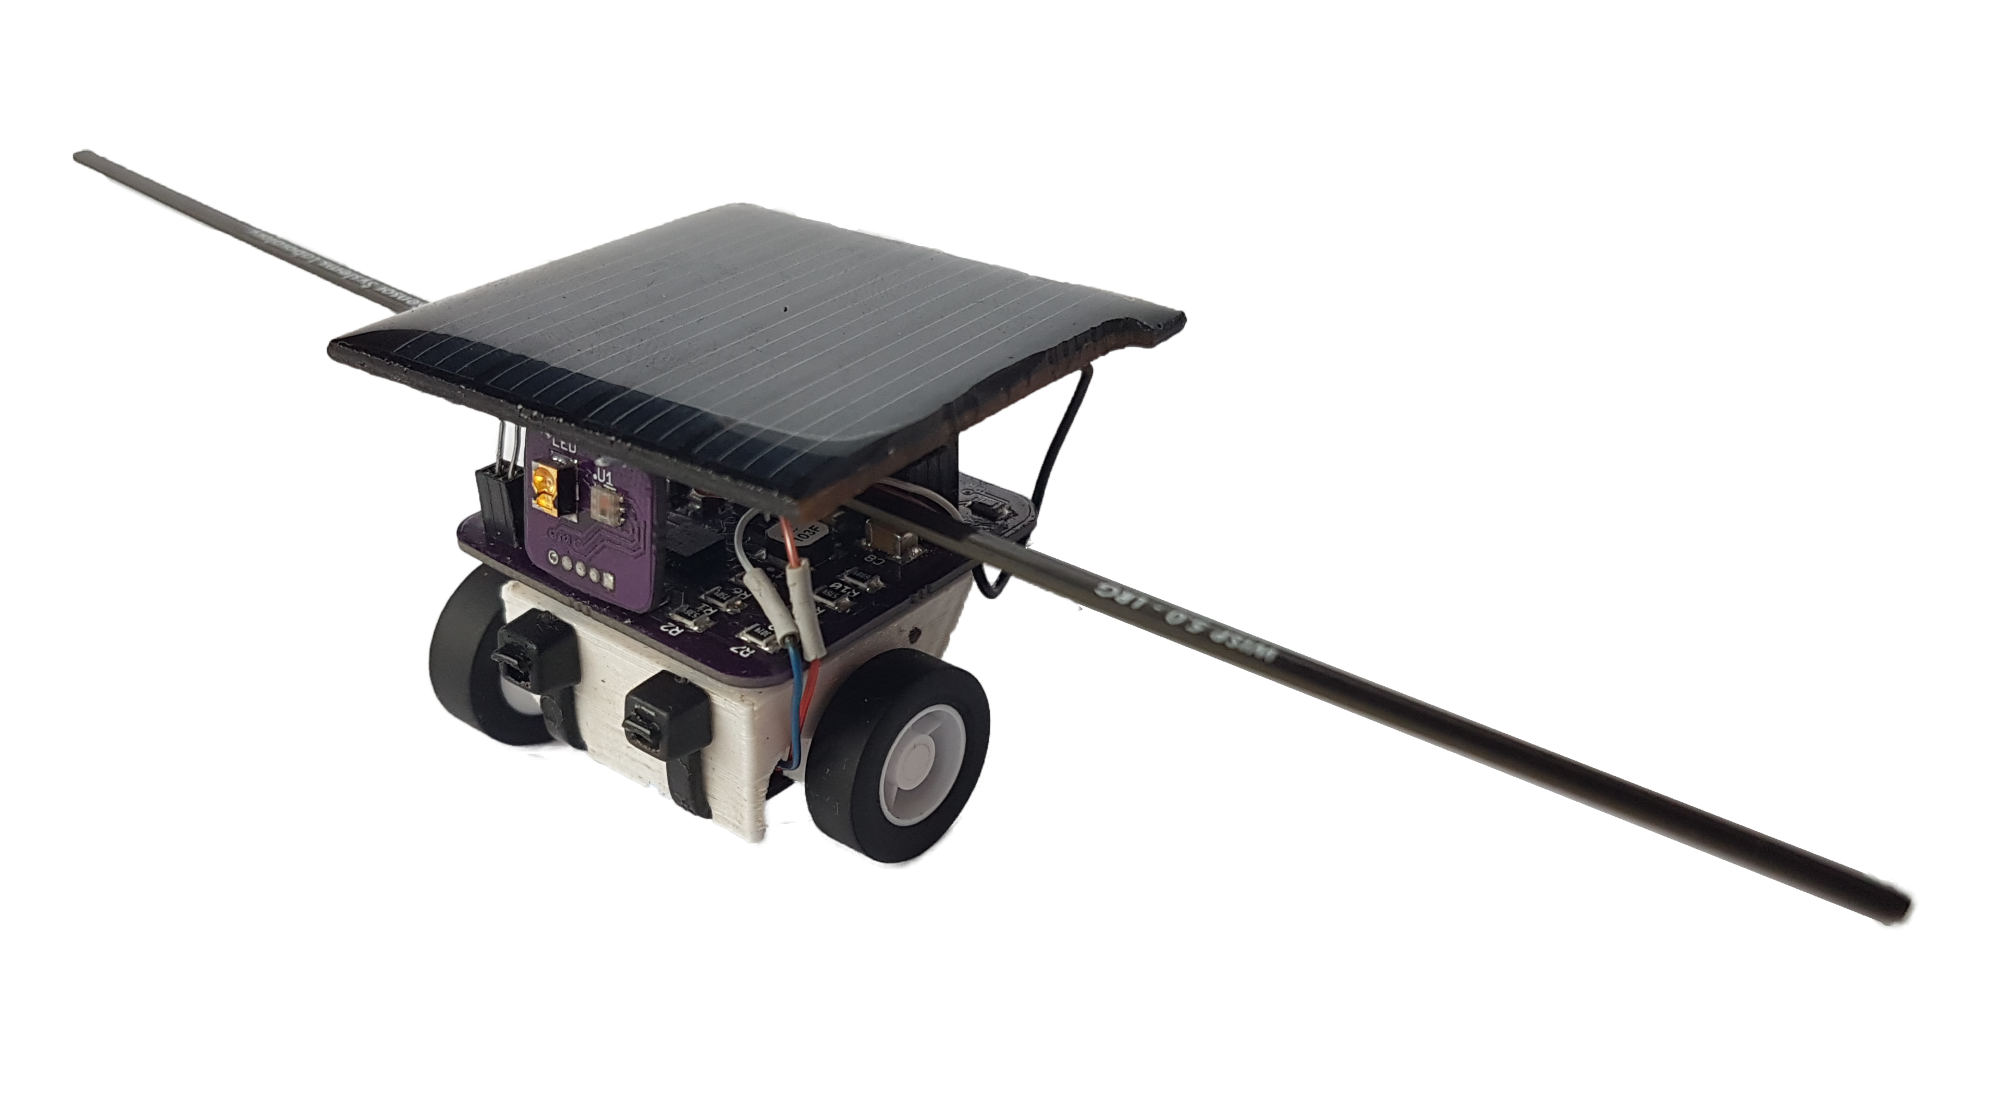
\includegraphics[width=13cm]{pics/tp_robot.png}
}
\vspace*{4cm}

\noindent
\hspace{1.89cm}
\hfill\parbox{5cm}{

\includegraphics[width=5cm]{pics/es_logo_cyan_black_rgb}}
\hspace*{2cm}\\

\vspace*{1.5cm}
\noindent

\includegraphics[width=\textwidth]{pics/TU_border_A4_L_front}
\end{textblock*}

\null\newpage


%%%%%%%%%%%%%%%%%%%%%%%%%%%%%%%%%%%%%%%%%%%%%%%%%%%%%%%%%%%%%%%%%%%%%%%%%%%%%%%
\hoffset=1.63cm
\oddsidemargin=0in
\evensidemargin=0in
\textwidth=5in

%%%%%%%%%%%%%%%%%%%%%%%%%%%%%%%%%%%%%%%%%%%%%%%%%%%%%%%%%%%%%%%%%%%%%%%%%%%%%%%
\parindent=1em

% EMPTY PAGE
\cleardoublepage

\pagestyle{plain}
\pagenumbering{roman}
\setcounter{page}{1}

% TITLE PAGE: page i (hidden)
\begin{titlepage}

  \begin{center}
  \null\vfill
    \begin{center}
    \LARGE{\reportTitle}
    \end{center}

    \vspace{3cm}

    \begin{large}
    Master's Thesis in \reportMSC
    \end{large}

    \vspace{1.5cm}

    \begin{normalsize}
    Embedded Software Section\\
    Faculty of Electrical Engineering, Mathematics and Computer Science\\
    Delft University of Technology\\
    Mekelweg 4, 2628 CD Delft, The Netherlands
    \end{normalsize}

    \vspace{2.0cm}

    \begin{normalsize}
    \reportAuthor \\
    \reportUrlEmail
    \end{normalsize}

    \vspace{1.0cm}

    % <MM> DD, YYYY
    \reportDate             %TODO: Dit is de datum van uitgifte van final versie aan de afstudeer commissie

  \vfill
  \end{center}

\end{titlepage}


% GRADUATION DATA AND ABSTRACT: pages ii and iii (hidden)
%De aankondiging bevat de spreker, titel, plaats, datum en tijd, samenstelling van de afstudeercommissie en een korte samenvatting (maximaal 25 regels).
\thispagestyle{empty}

\noindent \textbf{Author}\\
\begin{tabular}{l}
\reportAuthor{} (\reportUrlEmail)\\
\end{tabular}\\
\noindent \textbf{Title}\\
\begin{tabular}{l}
\reportTitle\\
\end{tabular}\\
\noindent \textbf{MSc presentation}\\
\begin{tabular}{l}
% <MM> DD, YYYY (like \today)
\presentationDate\\
\end{tabular}

\vspace{1.1cm}

\noindent \textbf{Graduation Committee}\\
\begin{tabular}{ll}
\graduationCommittee
\end{tabular}


\begin{abstract} %de abstract bevat alleen een korte samenvatting van de inhoud van het onderzoek
\setcounter{page}{3}
\reportAbstract{}
\end{abstract}

\clearpage

%\setcounter{page}{4}

% EMPTY PAGE: page iv
\cleardoublepage

% OPTIONAL QUOTATION: page v
%\pagestyle{empty}

\null\vfill

\begin{center}
\emph{``TODO QUOTE''} -- TODO QUOTED PERSON
\end{center}

\vspace{10cm}

\clearpage


% EMPTY PAGE: page vi
%\cleardoublepage

% PREFACE: page v
\chapter*{Preface}
\addcontentsline{toc}{chapter}{Preface}

This thesis presents the final work done towards obtaining my master’s degree in Embedded Systems from Delft University of Technology.
To the best of my knowledge no previous work has been conducted, exploring the feasibility of a transiently-powered battery-free robot. 


\vspace{1\baselineskip}

\noindent
I would like to express my sincere gratitude to my supervisor Przemys\l{}aw Pawe\l{}czak for his excellent guidance, never failing support and enthusiasm about this project. 
I also would like to thank Amjad Majid for letting me explore his idea of transiently-powered actuation, his constructive criticism and clever suggestions as this project evolved.
Moreover, I would like to thank Sinan Yildirim for his willingness to answer any of my questions, Ioannis Protonotarios for helping me with any hardware related issues, Michel Jansen for sharing his schematics.
Additionally, I would like to thank the Nuon Solar Team for lending me one of their space grade solar panels from their 2017 Nuna9 solar car.
Furthermore, I want to thank Prof. Koen Langendoen for hosting me at the Embedded Systems group, and Javier Alonso-Mora for participating as a member of my graduation committee.
Last but not least, a special thanks to my family for their unconditional support, encouragements and love that helped me stay motivated during this year.

\vspace{1\baselineskip}

\noindent
Koen Schaper

\vspace{1\baselineskip}

\noindent
Delft, The Netherlands

\noindent
\today

% EMPTY PAGE: page vi
\cleardoublepage

% TABLE OF CONTENTS: starting at page vii
\tableofcontents

\cleardoublepage

\pagenumbering{arabic}
\setcounter{page}{1}

% INTRODUCTION: page 1
\chapter{Introduction}
\label{chp:introduction}

% printer: Tethered flight control of a small quadrotor robot for stippling \cite{galea_iros_2017}

% Estabish your territory

Miniature robots with limited capabilities can work together in "swarms" to achieve more than an individual could by itself, but are still far from being applicable in real world applications~\cite{barca_sekercioglu_2013}.
The future potential of swarms is widely recognized to have applications in surveillance, search and rescue, and exploration.
Swarms have been proposed as a new form of user interface, robots can display information and interact with users on tabletops~\cite{legoc_uist_2016}, unmodified clothing~\cite{dementyev_uist_2016} and can be an educational toy for kids~\cite{sony_toio_2017}.
\hfill \break

% Establish nice
% Motivation for this work: Why do we want to remove the battery?

However, one of the fundamental issues that needs to be addressed before swarm robotics can advance is related to energy, small lithium batteries are currently powering the robots and limit their operation time to only a view hours. 
The energy density of batteries has improved less than 1 order of magnitude since 1945, in comparison the energy efficiency of computing has improved 12 orders of magnitude~\cite{patel_pvc_2017}.
The last major advancement in battery technology is 25 years old and came with the introduction of Li-ion batteries.
Additionally, any new big improvements in energy density of batteries is not likely to happen anytime soon, as new battery technologies are often overhyped and slow to emerge~\cite{zachary_spec_2016}.
\hfill \break

%TODO introduce current research

% Propose a solution: Energy harvesting
% And discuss current solutions to autonomus operation / battery replenishment

A stable energy supply is a current requirement to allow long term persistent autonomous operation of swarm robots.
Relaxing this constraint by allowing a transient supply of energy could be a potent area of research.
Wireless sensor nodes that rely on energy harvesting have already been emerging, some are highly energy constrained but fully eliminate the need for batteries.
In contrary, different replenishment methods for robot batteries are currently used, robots can be moved to a charging station leaving them nonoperational while recharging or the battery could be replaced, resulting in a high strain on maintenance.

% 4 lines left!
\newpage

\section{Problem statement}

% What why how

% Intermittently powered robots, that purely rely on harvested power are currently non existent.

Replacing a robots battery with an energy harvesting system could make it more self sufficient and energy-autonomous. 
This however introduces a new phenomenon to take into account; the intermittent availability of energy produces frequent power interrupts.
The possibility of sudden power loss is currently not considered when developing software that controls a robots behavior, and for this reason can not be used without adaption.
\hfill \break

Secondly, sensors and control techniques used may not be found applicable due to energy budget constrains or their inability to be interrupted by a loss of power. 
Different locomotion types are used and may not all be reliable and/or accurate under the frequent power interruption.
This research will explore the feasibility of a miniature battery-less robot, allowing persistent operation while being supplied with a small and intermittent source of energy.
Therefore the main question this work will try to answer is:

\begin{center}
	\textit{How to enable a transiently powered robot to operate autonomously?}
\end{center}

\section{Contributions}
Current swarm robots assume that a task can only be completed if sufficient energy is left in the batteries, which also limits their operation time. 
While surprisingly this is the first study of transiently powered robots, unaware of any platforms being implemented and are operating under the constant threat of power loss. 

\begin{enumerate}

%\item A simple model is developed showing the relation between the energy stored, weight of the robot, frequency of power cycles and distance covered with a single charge.

\item Design of a battery-less robot that purely operates from harvested energy, with basic capabilities allowing autonomous operation.

\item Implementation of a control algorithm, that allows the robot to finish a movement across power cycles.

%\item Evaluation of the battery-less robot compared to a battery powered robot in terms of, weight, speed and accuracy of movement.


\end{enumerate}


\section{Thesis Outline}
%What will be discussed in the coming chapters


\vspace{1\baselineskip}

\noindent
TODO ORGANISATIONAL DESCRIPTION OF THESIS



% CHAPTERS ... For instance: History/Prior Work, Design/Implementation, Experiments
\chapter{Related Work}
\label{chp:related_work}

This chapter will provide background information about current state of the art transiently powered systems. The advantages and disadvantages of different electrical storage types are compared. A short summary of current miniature robotics platforms is given and commonly used locomotion types. Finally different methods that try to ensure continuous operation will be discussed.

\section{Transiently-powered systems}
\label{sec:tp_systems}

% - Roughly everything that is powered fron a Energy harvester

Example of energy harvesting: Prolonged energy harvesting for ingestible devices~\cite{plonski_tranro_2016}
Drug delivery
\\
Converting a Plant to a Battery and Wireless Sensor with Scatter Radio and Ultra-Low Cost

%Other sources available for exploration are often limited by the application. Secondly, most sources can be scarce or completely absent during prolonged time intervals of the day as well \cite{RN15}. 

Fully programmable RFID platforms have been developed to exploring the combination of sensing, computation and communication, while allowing battery-less operation by harvesting RF energy~\cite{sample_transim_2008}.
The amount of energy collected from RF signals is very small and decreases with the distance of the device to the transmitter.
The harvested energy is typically stored in a capacitor, where larger capacitors can buffer more energy and smaller capacitors have the advantage of shorter charge times~\cite{gummerson_mobisys_2010}.
For longer, complex operations the energy budged needs to be evaluated carefully.
To store the energy an appropriate size storage capacitor needs to be selected~\cite{naderiparizi_rfid_2015}.

% - Short intro into persistent framwork: checkpointing etc
% mementos
% chain
% ratchet

\section{Energy Supply}
\label{sec:energy_supply}

% Explain battery vs supercapacitor

Comparing li-ion batteries with super-capacitors there are some big differences.
Supercapacitors do not need any special charging scheme and circuity for charging, except for overcharging protection.
Secondly, super-capacitors do not require any particular current profile, the energy can be stored at any rate and when the energy is required it can be extracted at any power level.
Operating a li-ion battery outside of it's recommended operating conditions can severely reduce a batteries lifetime and result in overheating or even explosion of the battery.
Batteries will seldom withstand more than one thousand complete charge/discharge cycles.
Super-capacitors used under extreme condition's, are not likely to explode but instead rupture.
While the biggest disadvantages of super-capacitors is their low energy density and high price, their lifetime is typically hundred thousands of charge/discharge cycles.

Li-Ion Battery-Supercapacitor Hybrid Storage System for a Long Lifetime, Photovoltaic-Based Wireless Sensor Network	\cite{ongaro_pwre_2012}
Reincarnation in the Ambiance: Devices and Networks with Energy Harvesting \cite{prasad_comst_2014}



\section{Small robotic platforms}
\label{sec:robotic_platforms}

%TODO tell that these robots are used for studing swarm behavior (inspired by nature)
% require communication to apply different algorithms
% need to be low cost and size are key factors for allowing scalability
% 
%Main characteristics : https://link.springer.com/article/10.1007/s11721-012-0075-2
%robots are autonomous;
%robots are situated in the environment and can act to modify it;
%robots’ sensing and communication capabilities are local;
%robots do not have access to centralized control and/or to global knowledge;
%robots cooperate to tackle a given task.

Low cost robotic platforms have been developed to tackle a variety of challenges anonymously.
Miniature robots can be used for inspection in difficult to reach places, operating like mobile sensing units.
Hardware modularity is a way to make the robot adapt its resources to different environments and sensing operations.
By separating out power, computation, motor control and sensing a verity of capabilities can be tested~\cite{sabelhaus_icra_2013, pickem_icra_2015, kim_iros_2016}.
Microrobots typically use infrared-based neighbor to neighbor distance sensing and communication~\cite{rubenstein_icra_2012, pickem_icra_2015, kim_iros_2016}.
While controlling a swarm or collective is mainly accomplished by means of active low power transceivers~\cite{sabelhaus_icra_2013, pickem_icra_2015, kim_iros_2016}. 

%TODO reference table

\section{Locomotion}
\label{sec:locomotion}
%TODO tell somthing about their accuracy!

Choosing the right locomotion resource can depend on different factors, moving in the most energy efficient way on a particular surface is often the determining factor.
On a flat surface, robots commonly use a two-wheeled differential drive design to not only move but allow for steering as well~\cite{sabelhaus_icra_2013, pickem_icra_2015}.
The GRITSBot does not use conventional DC motors, requiring encoders to estimate their speed. 
Instead by using stepper motors the speed can be set by changing the delay between steps. 
Estimating it's position therefore is reduced to simply counting steps~\cite{pickem_icra_2015}.  
Overall cost can be a decisive factor, therefore the Kilobot uses two vibrating motors for locomotion combined with three thin legs.
When the motors are activated the centripetal forces will generate a forward movement, which can be explained using the slip-stick principle~\cite{rubenstein_icra_2012}.
Other locomotion types are biologically inspired, the HARM-VP is small scale piezoelectric driven quadrupled robot~\cite{baisch_iros_2013}.
Each leg as two degrees of freedom, it can move up and down, as well as forward and backward.

\section{Continuous operation}
\label{sec:continous_operation}
%Battery replenishment

%TODO include battery tosti iron anecdote
Typically the operation time is extended by regularly checking the remaining energy in the battery and move to a recharging station before the robot runs out of energy~\cite{pickem_icra_2015, rubenstein_icra_2012}.
As an alternative to quickly recharging, the battery can also be swapped automatically when the robot moves into the docking station~\cite{kemal_mech_2015}.
Another work shows a robot which is able to swap it's primary battery using a six degree-of-freedom manipulator, used to grab the dead battery and plug it into a wireless recharging charging station \cite{zhang_conel_2013}.
Using direct wireless power to replace or supplement to a batteries energy is shown in~\cite{karpelson_icra_2014}, however the robot can only operate or recharge while remaining in close proximity to a transmitter. 
In these cases the robots are highly reliant on an infrastructure to allow for continuous autonomous operation.
This can be a severe constraint if the robot moves out of reach or needs to operate in a area where this infrastructure is not present. Persistent operation can also be achieved by harvesting renewable energy, particularly solar energy to complement to the robots internal energy source. To remove weight from the robot, in \cite{bruhwiler_iros_2015} the solar energy is used directly without any type of energy buffer. A drawback of this method is that the incoming solar energy should already greater or equal to the energy required for operation. This approach has been tested for basic locomotion and did not combine any form of sensing and control.

% - Provide overview table robots smaller than 15*15cm

% For each of these cases you need to provide numbers: 
% level of autonomy (does the robot does all by itself or relies on external processing)
% does autonomy fall under 
% charging time

% Add missing "new" robots

\begin{table*}[t]
	\centering
	\tiny
	\begin{threeparttable}
		\caption{An comparison of small robotic platforms}
		\label{tab:comparison_robot_platforms}
 		\begin{tabularx}{\textwidth}{l l X X X l l l} 
			\hline
 			Robot & Cost & Scalability & Sensors & Locomotion & Size [cm] & Weight [g] & Battery life \\ 
 			\hline
 			IPR & TBD & charge, program & gyro, distance, ambient light & wheel, 25cm/s & 4.0 & 21 & 1s\\
 			HAMR-VP\textsuperscript{1} \cite{bruhwiler_iros_2015} & NS & none & gyroscope, optical mouse & legged, 1cm/s & 4.4 & 2.3 & 3m \\
 			Roverables \cite{dementyev_uist_2016} & NS & charge & wheel, distance, optical encoders & wheel, ?? & 4.0 & ?? & 45m \\ 
 			Zooids \cite{legoc_uist_2016} & \$50 & ?? & position, touch & wheel, 50cm/s & 2.6 & 12 & 1-2h \\ 
 			mROBerTO \cite{kim_iros_2016} & \$60\textsuperscript{1} & program & light, range, gyro, camera, accel., compass, distance, bearing & motor shaft, 15cm/s & 1.5 & ?? & 1.5h\\
 			GRITSBot \cite{pickem_icra_2015} & \$50\textsuperscript{2} & charge, program, calibrate & distance, bearing, 3d accel., 3d gyro & wheel, 25cm/s & 3 & ?? & 1-5h \\
 			Kilobot \cite{rubenstein_icra_2012} & \$50\textsuperscript{2} & charge, program & distance, ambient light & vibration, 1cm/s & 3.3 & ?? & 3-24h\\
 			TinyTerp \cite{sabelhaus_icra_2013} & \$50 & none & 3d gyro, 3d accel. & wheel, 50cm/s & 1.8 & ?? & 1h\\
			\hline
		\end{tabularx}
		\begin{tablenotes}
			\item [1] Modified to include on-board power, sensing and control.
			\item [2] Cost of parts
		\end{tablenotes}
	\end{threeparttable}
\end{table*}

\chapter{Preliminaries}
\label{chp:preliminaries}

In this chapter the design considerations for the robot will be explained based on minimal required capabilities, in Section \ref{sec:pre_design_considerations}.
Section \ref{sec:pre_design_considerations} will evaluate two sources for energy harvesting and Section \ref{sec:pre_locomotion_selection} two types of locomotion for the transiently powered robot.
Finally in Section \ref{sec:pre_transient_model}, a simple model will capture the relation between power harvested and distance covered by the robot.

\section{Design Considerations}
\label{sec:pre_design_considerations}

This section will shortly explain the main areas considered while designing the battery-less transiently-powered robot

% - Optimize or low power consumption (disable or standby sensors and motor ctrl when not used)
% - Minimal basic functionality (for simple swarm algorithms?) (but no power hungry components ie optical encoders or mouse sensors)
% - Low power communication
% - Navigation

% Extra extra:
% - Tradeoff chargetime and operation time

\begin{enumerate}
	\item \textbf{Power}. 
	The robot should not rely on batteries, alternatively energy can be harvested from ambient sources and stored in a supercapacitor. 
	Energy harvested in a controlled environment should charge the capacitor in under 10 seconds and stored energy should provide at least an operation time of 1 second i.e. a minimal 10\% power duty cycle.
	
	\item \textbf{Small form factor}. 
	By making the robot as small as possible, weight is kept to a minimum reducing the energy required for movement.
	Secondly, designing the robot to use low cost off-the-shelf parts makes it convenient to build collectives of transiently-powered robots.
	
	\item \textbf{Locomotion}.
	Movement will consume the largest amount of energy from the total available energy budget.
	To optimize the distance that can be covered with a single capacitor charge, an efficient locomotion type needs to be selected for the movement on flat surfaces.
	
	\item \textbf{Autonomous navigation}.
	During operation the robot will experience a very frequent loss of power. 
	Despite regular power interruption the transiently-powered robot should be able to complete a movement with an acceptable error when compared to its battery powered equal.
	
	%TODO write about ability to expand to swarming
\end{enumerate}

\section{Energy Source Selection}
\label{sec:pre_energy_source_selection}
% RF harvesting seems prommesing
% Wispcam requires approx 4 seconds to harvest 20mJ at a distance of 20cm from the reader \cite{naderiparizi_rfid_2015}
% better to only use RF for communication and harvest energy from another source \cite{konstantioulos}

In this section the charge time of two different sources of ambient energy will be compared, RF and Solar.
To determine which source is the most suitable for powering the transiently-powered robot, their performance will be evaluated for different distances.
The average input power will be determined from the time to charge a capacitor as

\begin{equation}
	P_{\text{in}} = \frac{E_{\text{cap}}}{t_{\text{charge}}}
\end{equation}

\noindent
where $E_{\text{cap}}$ the energy stored in a capacitor and $t_{\text{charge}}$ the average charge time.
The energy stored in a capacitor given a minimum and maximum voltage level can be defined as

\begin{equation}
\label{eqn:energy_cap}
	E_{\text{cap}} = \frac{1}{2}C(V_{\max} - V_{\min})^{2}
\end{equation}

\noindent
where $C$ is the capacity of a the capacitor, $V_{\min}$ the minimum and $V_{\max}$ the maximum voltage level of the capacitor.

\subsection{Energy Harvesting and Storage}
\label{sec:pre_energy_harvesting_storage}
Energy is harvested using a Texas Instruments BQ25570 energy harvester~\cite{bq25570_2017}, which includes a nanopower boost charger with maximum power point tracking to extract the optimal amount of energy. 
The harvested energy is stored in a 22\,mF - 4.5\,V supercapacitor from AVX~\cite{avx_bestcap_2017}, chosen for its low leakage current and small size.
The Texas Instruments BQ25570 has a buck converter to efficiently regulate the capacitors voltage down to the system voltage of 2.2\,V.
External resistors are used to program voltage thresholds, allowing to automatically enable and disable the buck converter based on minimum and maximum thresholds.
The minimum threshold is set to 2.2\,V and the maximum threshold is set to 4.2\,V.
Using Equation \ref{eqn:energy_cap} the energy stored in the capacitor can be determined to be equal to

\begin{equation}
\label{eq:cap2}
E = \frac{1}{2} 0.022 (4.4 - 2.2)^2 = 53.24 mJ
\end{equation}

%Additionally the resistors are used to set the overvoltage protection and the buck converter output voltage.
%The minimal supply voltage is determined by the component with the highest minimal voltage requirement, in this case 2.0\,V.
%To make sure that a small drop in system voltage would not create instability a margin of 0.2\,V was added, resulting of a system voltage of 2.2\,V.

\subsection{Determining the Charge Time}

The buck converter of the energy harvester is automatically enabled when the maximum voltage threshold is reached.
A load is connected to the output of the buck converter to quickly drain the energy from the capacitor.
In this case load is chosen such that the power consumed by the load $P_{\text{load}} >> P_{\text{in}}$.
By connecting a Saleae logic analyzer~\cite{saleae_2017} to the output of the buck converter, the period of the power cycles can be recorded.
The time that the output of the buck converter is disabled will be equal to the time to charge the capacitor from the minimum to the maximum threshold.

\subsection{Energy Harvesting from RF}

\subsubsection{Harvesting using a WISP}
To be able to connect an external harvester, a WISP 5~\cite{sample_transim_2008} was modified.
The integrated energy harvester, the storage capacitor and the diode to bypass the harvester, were removed from a WISP.
A wire was soldered to the input pin pad of the now removed harvester on the WISP PCB.
This wire was connected directly to the input of the external energy harvester.

\subsection{Measurements}
Energy was provided to the WISP using a Impinj Speedway R1000 RFID reader~\cite{impinj_eol_2017, indy_r1000_2017}.
This reader was connected to a Laird S90028PCR antenna~\cite{laird_s9028pcr_2017}.
The WISP is positioned 25, 35 and 45\,cm away from the reader and the charge time was recorded.

\begin{table}[t]
	\centering
	\caption{The average charge time with RF}
	\label{tab:res_rf_harvest}
	\begin{tabular}{|l||l|l|l|}
		\hline
		Distance & 25\,cm & 35\,cm & 45\,cm \\
		\hline \hline
		Average charge time & 49.1\,s & 61.1\,s & 164.8\,s \\
		%Average input power & 1.086\,mW & 0.871\,mW & 0.323\,mW \\
		\hline
	\end{tabular}
\end{table}

\subsubsection{Results}
The time to charge the capacitor is more than 49\,s, see Table \ref{tab:res_rf_harvest}.
As the WISP is placed further away from the reader the charge times increase significantly.
While the distance increases more power is directed away from the WISP due to reflections of the signal.

\subsection{Energy Harvesting from Light}

In this section the charge time of small solar panels under different light sources is evaluated.
Sunlight is not always available or enough to charge the robots in a acceptable time.
A lighting setup needs to be created that provides a reasonable amount of uniform light to the area where the robot moves around.
To accurately measure the power that is harvested from each solar panel, their performance was evaluated in a darkroom at TU Delft Embedded Software Lab.

\subsubsection{Solar panels}
Three different solar panels were tested, each different in material, efficiency and panel size, as can be seen from Table \ref{tab:solar_panels}.

\begin{table}[t]
	\centering
	\resizebox{\columnwidth}{!}{%
		\begin{threeparttable}
			\caption{Specification of the solar panels tested in the experiment.}
			\label{tab:solar_panels}
			\begin{tabular}{|l|l|l|l|}
				\hline
				& Material & Efficiency (\%) & Dimensions (mm) \\
				\hline \hline
				Banggood~\cite{bangood_solar_2017}& Poly-Si & 17 & 40x30 \\
				INYS SLMD121H04L-ND~\cite{ixolar_slmd121h04l_2017}\textsuperscript{1}& Mono-Si & 22 & 43x34 \\
				Azurspace 3G28C~\cite{azurspace_3g28c_2017}& Triple Junction GaAs& 28 & 80x40 \\
				\hline
			\end{tabular}
			\begin{tablenotes}
				\small
				\item [1] Two panels in parallel
			\end{tablenotes}
		\end{threeparttable}
	}
\end{table}


\subsubsection{Lamps}
Low cost solar simulators can consist of a combination of LED and halogen light bulbs to simulate sunlight and are used to test the performance of solar panels~\cite{grandi_tia_2014}.
However, in this case the goal is to have a controlled uniform lighting environment where the robots have roughly constant charge times.
Solar panels do not only harvest energy from the visual light spectrum but harvest almost at least as much from the infrared light spectrum, therefore not only light but also heat will shorten the charge time~\cite{ixolar_slmd121h04l_2017}.
Halogen lamps have a lower color temperature than the sun but also emit waves far into the infrared spectrum.
The light sources used in this experiment are a 60\,W halogen bulb, a 120\,W halogen halogen bulb and two 150\,W Philips  BR125, infrared (IR) incandescent reflector lamps~\cite{philips_irlamp_2017} where one is clear and the other uses a red filter.

\subsubsection{Measurements}
Three charge time measurements were preformed, each lamp was positioned 10\,cm, 30\,cm and 50\,cm from the solar panels.
To have a reference the charge times were also measured on a sunny afternoon. 
% Additionally, for these three distance the temperature was measured at the solar panel using a K-type thermocouple supplied with an Extech EX330 multimeter and the light intensity using the luxmeter on a MASTECH MS8229 multimeter.

\subsubsection{Results}
% No difference between the heatlamps in power consumed
% Halogen distributes the light more even
% Panel from nuna
% Refer to appendix for temperature and light data?

Increasing the output power of the source and decreasing the distance between panel the source, both decrease the charge times.
However, there is no clear winner as seen from Table \ref{tab:light_results}.

Something to take into consideration is that with some lamps a shadowing pattern is observed due to the construction of the lamps.
The 60\,W and 150\,W IR lamps have a spherical design, that creates a uneven circular shadowing pattern on the surface the lamps are shining on. 
This becomes more significant on the bigger distances in this experiment.
The 120\,W halogen lamp has a tubular design and in combination with the light fixture most of the light is reflected down with minimal shadowing of the lamp resulting in a more even light distribution.
Therefore, this lamp is chosen to provide light in the controlled setup where the robots can move around with roughly constant charge times.

For this lamp on the distances 30\,cm and 50\,cm the Azure space solar panel seems to preform the best.
However, the surface area of this panel is more than double when compared to the other two solar panels, as seen from Table \ref{tab:solar_panels}.
Therefore the charge times should be doubled, which makes the INYS panel the best performer.

Additionally the charge times were recorded for each solar panel during a sunny, blue sky, November afternoon, as seen from Table \ref{tab:solar_results}.
The Azurspace solar panel is in this case the winner as, this was expected as it has is able to harvest energy from the broadest part of the light spectrum.

%Both the temperature and illumination increase by decreasing the distance between the light source and the solar panel. 
%Secondly, increasing the output power of the lamp increases temperature and illumination as well. 

\begin{table}[t]
	\centering
	\caption{The average charge times in seconds for different distances from the sources.}
	\label{tab:light_results}
	\begin{tabular}{|l|l||l|l|l|l|}
		\hline
		\multicolumn{2}{|c|}{} & \multicolumn{4}{|c|}{Source} \\
		\hline
		Distance (cm) & Panel & 60\,W & 120\,W & 150\,W clear & 150\,W red \\
		\hline \hline
		\multirow{3}{*}{10} & Banggood & 3.08 & 2.19 & 0.99 & 0.73 \\
		& INYS & 2.76 & 0.82 & 0.51 & 0.56 \\
		& Azurspace & 2.81 & 1.61 & 0.77 & 1.77 \\
		\hline
		\multirow{3}{*}{30} & Banggood & 6.45 & 6.72 & 7.83 & 1.88 \\
		& INYS & 8.76 & 6.21 & 2.92 & 1.63 \\
		& Azurspace& 11.53 & 4.12 & 9.88 & 10.16\\
		\hline
		\multirow{3}{*}{50} & Banggood & 26.28 & 17.59 & 17.91 & 9.46 \\
		& INYS & 49.70 & 17.00 & 10.15 & 7.63 \\
		& Azurspace & 53.33 & 12.09 & 23.1 & 46.96 \\
		\hline
	\end{tabular}
\end{table}

\begin{table}[t]
	\centering
	\caption{Charge time from solar.}
	\label{tab:solar_results}
	\begin{tabular}{|l|l|}
		\hline
		Panel & Charge time (s) \\
		\hline \hline
		Banggood & 3.84\\
		INYS & 3.89\\ 
		Azurspace & 1.40\\
		\hline
	\end{tabular}
\end{table}

\subsection{Conclusion}

The results from RF experiments show that the minimum charge time is 49\,s and more than doubles with only a 20\,cm distance increase from the reader.
The mobility of the robot will result in widely varying charge times and possible dead spots where the robot is not able to receive any power.
Light is more readily available and by illuminating the area where the robot moves around with a 120\,W halogen source shows 6\,s charge times when positioned 30\,cm from the solar panel.
With the solar panel far shorter charge times can be achieved, and therefore solar is chosen to be the energy source for the transiently powered robot.

\section{Locomotion Selection}
\label{sec:pre_locomotion_selection}

Robots can use dead reckoning to move between locations without external feedback, but in order to accomplish this accurate locomotion and basic odometry are required.
In this section two different locomotions types will be evaluated, the stepper motor and the DC motor.
%TODO Move this part!
%TODO DEFINE AND REFERENCE
%Wheel encoders are often used to determine the angular speed of each wheel, which can be used to correct speed differences between the motors and can be integrated over time to acquire distance.
%Miniaturizing encoders significantly reduces their resolution, and can be classified as power hungry when considering a small energy budget and active light source is used.
%TODO NEED REFERENCE FOR THIS CLAIM

\subsection{Stepper motor-based Locomotion}

The GRITSBot~\cite{pickem_icra_2015} uses stepper motors based locomotion which already include basic odometry, as described in Section \ref{sec:rw_locomotion}.
This section will further investigate the use of stepper motor based locomotion for a transiently-powered robot.

\subsubsection{Operation of a Stepper Motor}
Stepper motors are permanent magnet dc motors that start to rotate by supplying current to the motor coils in a specific direction.
The bipolar stepper motor used, requires current to be pulsed trough each of the four connections, in a fixed pattern, in order to rotate it forward or backward.
A Microcontroller (MCU) is used to keep track and instruct the next stepper motor position from a sequence of four.
The outputs of the MCU cannot supply enough current to drive a bipolar stepper motor, therefore a dual H-bridge is required to control the current trough each coil.

%TODO make new schematic stepper figure!
%http://homemaderobo.blogspot.nl/2012/03/stepper-motor.htm
\begin{figure}
	\centering
	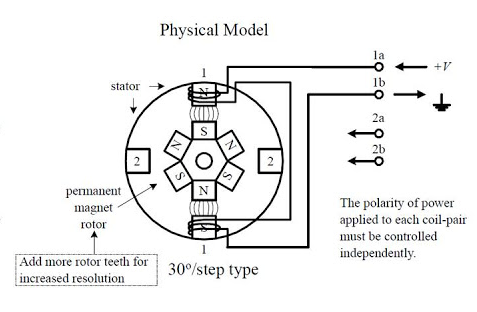
\includegraphics[width=\textwidth]{pics/bipolar_stepper.png}
	\caption{Need better / simpler figure here!}
	\label{fig:bipolarstepper}
\end{figure}

\subsubsection{Current Consumption}
%TODO values that calculate the current per motor?
%TODO ADD CURRENT MEASUREMENTS @ 2.2 v
The current consumed by a stepper motor is constant and independent of the angular velocity of the rotor.
The average current consumed is equal to: $\textrm{I} = V_{\text{supply}}/R_{\text{coil}}$.
Therefore running the motor at maximum speed, translates the most electrical energy into kinetic energy.
However, the motor speed is inversely proportional to the motor's output torque and therefore the maximum speed is limited by the minimal required output torque.
%The current trough the coils is constant, so the faster the stepper motor changes step the more energy can be transformed into movement.
%Increasing the rotational speed of the stepper motor decreases the torque output of the motor.
%Therefore the speed is limited by the amount of torque required to preform the movement.

\subsubsection{Control and Rotor Synchronization}

The only way to grantee that the teeth on the rotor will stay aligned with the coil, is to keep the coil energized until the next position is instructed and succeeding coil is energized. 
On the first startup the rotor may not be aligned with the last position in the sequence of four.
As a result an error between one and three steps can occur before the energized coil and rotor are synchronized.

In case the stepper motor is rotating and the power is removed, misalignment between the rotor and the last energized coil can occur.
While the rotor could be moving from one position to the next, it has not moved at all (undershoot) or can continue to move to the next position due to inertia of the rotating mass (overshoot). 
To determine what would be more likely, undershooting or overshooting, the following experiment has been preformed to determine the error in the number of steps.

\subsubsection{Experimental setup}

Tiny 6\,mm permanent magnet bipolar stepper motors from Nidec are frequently used in digital camera's~\cite{nidec_stepper_2017}.
For this motor one rotation is equal to 20 steps i.e five times the sequence of four.
This stepper motor is suspended and a needle glued to the motor shaft.
The needle rotates over a round piece of paper which is divided by markings in 20 steps.%, as seen from Figure \ref{fig:step_counting}.
First the rotor and coil are synchronized by moving four steps, and the position of the needle is visually recorded and written down.  
Then the stepper motor is commanded to make one rotation equal to 20 steps.
After rotating 20 steps the power is removed from the coils and the needle position is again visually recorded and written down.

\begin{figure}
	\centering
	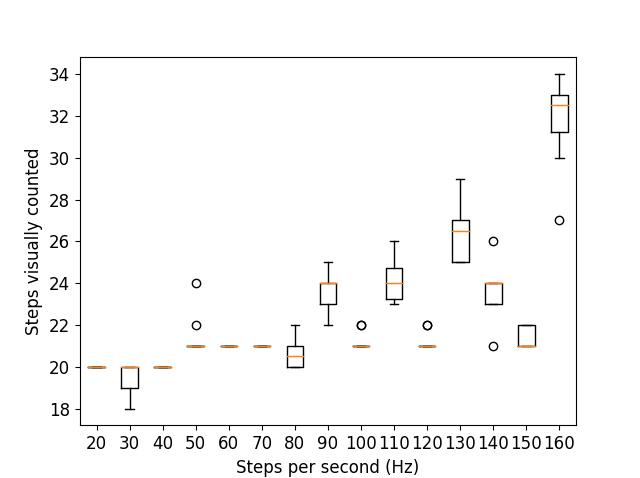
\includegraphics[width=0.8\textwidth]{pics/figure_intertia.png}
	\caption{Stepper motor inertia result}
	\label{fig:step_results}
\end{figure}


%\begin{subfigure}[b]{0.38\textwidth}
%	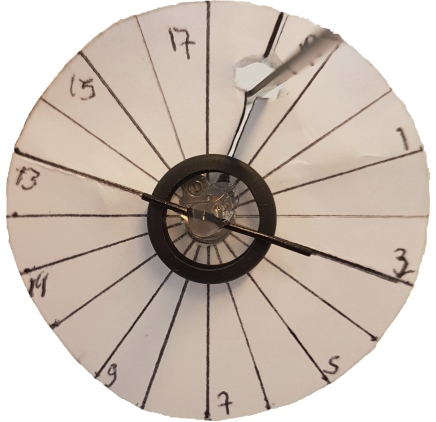
\includegraphics[width=\textwidth]{pics/step_counting.jpg}
%	\caption{Experimental setup for determining error in the number of counted steps}
%	\label{fig:step_counting}
%\end{subfigure}	


\subsubsection{Stepper Motor Inertia Result}

Figure \ref{fig:step_results} shows the result of the experiment.
The stepper motor on average will overshoot, i.e. will do more steps than commanded when the power is removed.
This effect is becomes more significant with increasing step frequency.
However, while this experiment only shows the effect for an unloaded motor, it is likely that a synchronization error will occur when a transiently-powered robot would be powered using two stepper motors in differential drive.
After every power interrupt each motor first needs to be synchronized, which will result in the robot making a random turn if the error between the motors is not equal.

\subsection{DC Motor locomotion}
\label{sec:pre_dc_motor_locomotion}
Small dc motors are commonly selected to provide locomotion for small robotic platforms as seen from Table \ref{tab:comparison_robot_platforms}.
In this section the DC motor will be evaluated as the locomotion type for the transiently-powered robot.

\subsubsection{Operation of a DC Motor}

When voltage is applied to the motor, current rises as quickly as the inductance in the motor windings allows.
DC motors produce an initial startup peak because the back electromotive force (back EMF) is initially zero.
The current reaches a maximum when the rotor starts to rotate and a back EMF is generated.
The back EMF will further increase while the motor accelerates to its steady state speed, and the speed is limited by the voltage supplied.

If a load is applied to the DC motor the current consumed by the motor is increased because current is proportional to the torque applied to the motor.
Additionally, the angular velocity of the motor will decrease while the torque is inversely proportional to the angular velocity of the motor.

\subsubsection{Evaluation of the Start Current Peak}
The DC motors used for robots are normally powered directly from the battery as linear or switch-mode power regulators are not able to supply the high start currents.
%In the worst case the start current peak can be equal to the stall current of the motor.
However, the use of a supercapacitor requires a regulator to make efficient use of the energy stored, as described in Section \ref{sec:pre_energy_harvesting_storage}.
The switch-mode regulator that is part of the BQ25570 energy harvester is only able to supply a peak output current of 110\,mA~\cite{bq25570_2017}.

%To evaluate the magnitude of the current peak, the free running current profile of 
The 206-11 DC motor from Precision Microdrives~\cite{gearmotor_206-110_2017} is the selected motor that will be evaluated.
From the datasheet a typical start current of 185\,mA can be found for its rated operating voltage of 3\,V.
However, the system voltage chosen for transiently-powered robot is 2.2\,V.
To determine the startup current of a 206-110 motor when supplied with 2.2\,V, a two second current trace is recorded using a Monsoon Power Monitor~\cite{monsoon_powermonitor_2017}.


\begin{figure}%[h!]
	\centering
	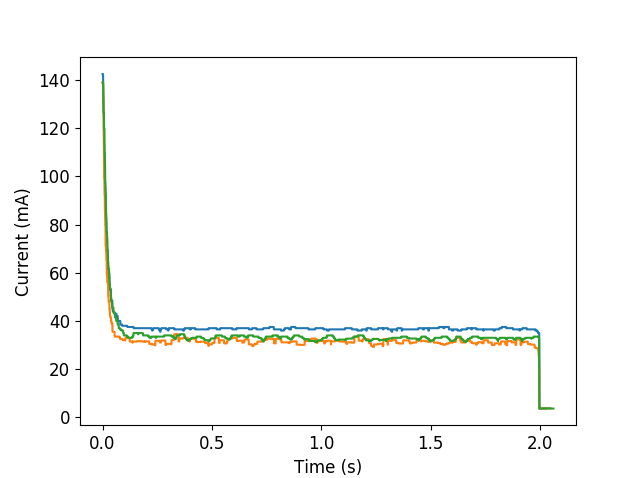
\includegraphics[width=0.62\textwidth]{pics/free_running_current.png}
	\caption{Current profile of the dc motor.}
	\label{fig:free_running_current}
\end{figure}

\subsubsection{Results}
The measurement results for three different motors is shown in Figure \ref{fig:free_running_current}
The results show that the 2.2\,V supply voltage reduces the start current peak to 140\,mA.
This is still above 110\,mA and the robot needs to power two motors in a differential drive configuration to allow steering.
A solution is to use Pulse Width Modulation (PWM) to reduce the motor speed and average current consumed.
Combining PWM with a large bulk capacitor should enable the buck converter to start the motors.
However the PWM duty cycle will be limited to a maximum of $100/(2*140/110) \approx 39\%$, and will be further reduced by the load applied to the motors as a result of the robots own weight.


\subsection{Conclusion}
Stepper motor have a lower efficiency than normal dc motors because a constant current consumed independent of the rotational speed.
The only way the rotor and stator retain alignment is by keeping the stepper motor coil energized.
Very frequent power interrupts could lead to loss of synchronization between the energized coil and position of the rotor as a result of rotor inertia.
The error due to inertia becomes more significant with increase rotational speed.
Loss of synchronization can result in random behavior of a differential drive robot, as one stepper motor may require a different amount of steps before synchronization than the other.

Alternatively a normal DC motors can be used which do not require any synchronization.
However, this motor requires a high start current which the buck converter from the harvester, might not be able to supply.
PWM can be used to reduce the average current consumed by the motor and a large bulk capacitor can supply short high current demand from the motors.
Therefore the dc motor is chosen as the locomotion type used for the transiently-powered robot.

\section{Transiently-powered Robot Model}
\label{sec:pre_transient_model}

In this section a simple model will be derived showing the relation between size and weight of the robot, the amount of power that is harvested and stored and how much of this can be translated into linear movement.

\subsection{Modeling Assumptions}

Energy is harvested from an ambient source and stored in a supercapacitor.
To make efficient use of the energy stored in a supercapacitor a regular is required to supply a stable voltage to the connected loads.
In this case the loads are two identical dc motors which each drive wheel. \\
\\ \noindent
The following assumptions will be used to model the transiently powered robot:
\begin{itemize}
	\item The required power by the loads is greater than the incoming power, resulting in repeated power cycling of the robot.
	\item The amount of input power after conversion is constant due to the use of a controlled environment
	\item Since a regulator is used, the voltage in the capacitor will never fall below the operating voltage.
\end{itemize}

%The input power Pin, will be stored in a supercapacitor with capacitance C.


%The regulated output voltage is a lower threshold for the energy that can be used from the capacitor.
%The upper threshold is determined by the maximum voltage rating of the supercapacitor.
%Lowering the output voltage allows for more energy to be used from the supercapacitor, and also lowers the overall power consumption of individual components.
%The energy stored in supercapacitor is a function of the capacitance and the threshold voltage difference, being equal to:








% 1 Incomming power V * I which scales with solar panel size

% 2 Maximum power point tracking (switchmode boost converter)

% 3 Stored in non-ideal supercapacitor with capcitiy C and a parrallel resistance Rleak and series resistance (ESR, typically small but not neglectable?)

% 123 determine chargetime

% Buck converter losses 

% Power consumed from source = Pcons = Ploss + Pweels

% Power P(t)  = F * v = T x omega

\subsection{Motor Dynamics}

The electrical equivalent circuit of a brushed dc motor is shown in Figure \ref{fig:pre_model_dc}, where $v$ is the voltage applied to the motor, $i$ the armature current, $R$ the armature resistance, $L$ the armature inductance, $e$ the back EMF voltage, $\tau$ the torque produced by the motor, $\omega$ the angular velocity of the rotor, $J$ is the moment of inertia of the rotor, $B$ is the viscous friction coefficient of the motor bearings and $m$ the external applied torque.


\begin{figure}[h!]
	\centering
	\begin{circuitikz}
		%\draw [help lines] (-1,-2) grid (12,5);
		
		% electrical equivalent circuit
		%\draw (0,0) to[V, v_=$v$] (0,3);
		\draw (0,3) node[ocirc] {}; % ,label=left:+
		\draw (0,3) to[R, i>^=$i$, l=$R$] (3,3);
		\draw (3,3) to[L, l=$L$] (4,3);
		
		\draw (0,2.25) node {$+$};
		\draw (0,1.5) node {$v$};
		\draw (0,0.75) node {$-$};
		
		\draw (4,3) -- (5,3);
		\draw (5,3) -- (5,2);
		%\draw (5,1.5) node[elmech](motor){M};
		\draw (5,1) -- (5,0);
		
		\draw (4.25,2.25) node {$+$};
		\draw (4.25,1.5) node {$e$};
		\draw (4.25,0.75) node {$-$};
		
		\draw (0,0) -- (5,0);
		\draw (0,0) node[ocirc] {}; 
		
		% motor
		\draw[fill=white] (4.85,0.85) rectangle (5.15,2.15);
		\draw[fill=white] (5,1.5) ellipse (.45 and .45);
		
		
		% shaft drive -> transmission
		\draw[fill=black] (5.45,1.45) rectangle (7.0,1.55);
		
		% momentum arrow of drive -> transmission
		\draw[line width=0.7pt,<-] (5.8,1) arc (-30:30:1);
		
		% moment of inertia
		\draw[fill=white] (7.5,1.59)
		ellipse (.15 and 0.4);
		\draw[fill=white, color=white] (6.9, 1.99)
		rectangle (8.49, 1.19);
		\draw (6.8,1.59) ellipse (.15 and 0.4);
		\draw (6.8,1.99) -- (7.5,1.99);
		\draw (6.8,1.19) -- (7.5,1.19);
		
		% momentum arrow (left hand side of brake shoe)
		\draw[line width=0.7pt,->] (8.05,1.1) arc (-30:30:1);
		
		% descriptions inside graphic
		\draw (5.85,2.2) node {$\omega_A, M_A$};
		\draw (7.25,1.61) node {$J$};
		\draw (8.05,2.32) node {$M_R$};
		
	\end{circuitikz}
	\caption{Brushed DC motor system model.}
	\label{fig:pre_model_dc}
\end{figure}

\noindent
Using Kirchhoff's voltage law the electrical dynamics of a dc motor can be described as
\begin{equation}
\label{eq:kirchhoff}
v = Ri + L \dot{i} + e
\end{equation}

\noindent
From Newton's second law follows that the mechanical dynamics of a motor can be described as
\begin{equation}
\label{eq:newton}
\tau = J\dot{\omega} + B\omega + m
\end{equation}

\noindent
The electromechanical equations state that the back EMF voltage is proportional to the angular velocity and the motor torque is proportional to the armature current

\begin{equation}
\label{eq:electomechanical}
\begin{gathered}
e = k_{e} \omega \\
\tau = k_{t} i
\end{gathered}
\end{equation}

\noindent
where $k_{e}$ is the back emf constant of the motor and $k_{i}$ the torque constant of the motor.
The electrical power consumed and mechanical power consumed will be equal to

\begin{equation}
\begin{gathered}
p_{\text{e}} = vi \\
p_{\text{m}} = \tau\omega
\end{gathered}
\end{equation}

\noindent
Rewriting equation \ref{eq:kirchhoff}, \ref{eq:newton} and \ref{eq:electomechanical} and appling the Lalace transa transfer function from $v$ to $\omega$ can be obtained, assuming $m$ = 0.

\begin{equation}
\frac{\Omega(s)}{V(s)} = \frac{k_{i}}{(Ls + R)(Js + B) + k_{\omega}k_{i}} 
\end{equation}

where $V(s)$ and $\Omega$ are the Lapace transformations from $v$ and $\omega$ respectively.


\subsection{Robot Dynamics}
The robot is modeled as a mass $m$, that is moved by two wheels with radius $r$, each connected directly to a motor.


The rolling friction between the wheels and the surface is equal to:
\begin{equation}
F_{\text{k}} = \mu_{\text{k}}mg
\end{equation}

Therefore the torque applied to the motor due to rolling friction, as it is only present while the robot is moving relative to the surface and the equation becomes:

\begin{equation}
T_{\text{ext}} = rF_{\text{k}} sgn(\omega)
\end{equation}

\noindent
The total mass is equal to the 

%
\section{Modeling a Transiently-powered Robot}
\label{sec:design_requirements}

% 1 Incomming power V * I which scales with solar panel size

% 2 Maximum power point tracking (switchmode boost converter)

% 3 Stored in non-ideal supercapacitor with capcitiy C and a parrallel resistance Rleak and series resistance (ESR, typically small but not neglectable?)

% 123 determine chargetime

% Buck converter losses 

% Power consumed from source = Pcons = Ploss + Pweels



\chapter{Design and Implementation}

% - Should the subsections more or less reflect the columns in the table?

\section{Hardware Design}

% - EXPLAIN MORE ABOUT HARDWARE CHOISES, why these specific componens. What were the requirements for choosing these components

The first step was to evaluate what components are required for the robot to have basic navigation capabilities.
Commercially available low power components have been evaluated, where the main criteria was a low minimal supply voltage.
This section will explain each part of the robot in more detail and a complete overview of the robot is shown in Figure \ref{fig:robot_overview}.

\vspace{1em}
\begin{figure}[h!]
	\centering
	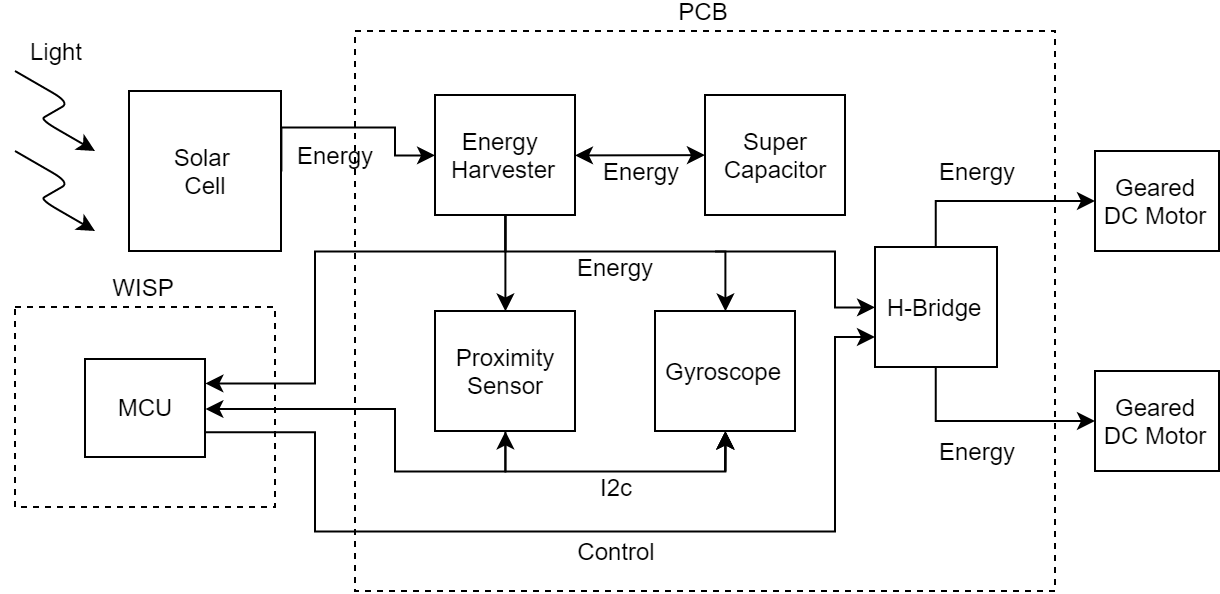
\includegraphics[width=\textwidth]{pics/schematic_robot_v2.png}
	\caption{Schematic overview of the robot.}
	\label{fig:robot_overview}
\end{figure}

\subsection{Energy Source}
%TODO refer to preliminaries section
Solar energy is harvested from two IXYS SLMD121H04L-ND solar cells~\cite{ixolar_slmd121h04l_2017} in parallel.
These monocrystalline solar cells have a high efficiency of 22\%, allowing energy harvesting even in low light conditions.
The solar cells are connected to a energy harvester. 

\subsection{Computation}
\label{sec:dai_computation}

The robot is designed around a WISP 5 \cite{wisp5_wiki_2017}, a battery-free platform for low power sensing, computation and communication.
This platform has the ability to communicate with RFID readers and is powered by the carrier signal emitted by the reader.
However, the communication range and the power that can be harvested is limited.
Therefore communication is currently not implemented and a different energy source for harvesting will be used as described in Section \ref{sec:pre_energy_harvesting_storage}.
Currently only the MCU from the WISP is being utilized: a Texas Instruments MSP430FR5969 ultra low power microcontroller.
This MCU can operate at 16\,MHz and features 64\,KB FRAM, 2\,KB SRAM and 40 IO-ports \cite{msp430fr5969_2017}.

\subsection{Sensing}
\label{sec:dai_sensing}

The robot has access to basic sensors which can be interfaced trough I2C.
For detecting obstacles in front of the robot, a Maxim Integrated MAX44000 proximity sensor was added of the robot facing forward.
This sensor switches a IR led at high frequency to reduce the power consumed.
The same sensor is based around a photo-diode it can be used to measure the amount of ambient light as well.
To allow for controlled movements the robot has a Bosch Sensortec BMG250 low power triaxial gyroscope to measure yaw-rate, used to correct it's heading when necessary.

\subsection{Locomotion}

% tell that also higher geared motors were tried??

Two 25:1 sub-micro plastic planetary gearmotors from Precision Microdrives~\cite{gearmotor_206-110_2017} are mounted in a 3D printed frame.
The motors are positioned diagonally opposite from each other making the robot as compact as possible, while this differential drive configuration allows the robot to steer.
Small plastic wheels with rubber tires are mounted directly on each of the motor shafts.
Behind these two motors a free running caster wheel is mounted to the frame, acting as a third support point for the robot.

\subsection{Motor Control}
\label{sec:dai_motor_control}

The speed (and the current consumption) of each motor can be controlled individually using Pulse-Width-Modulation (PWM).
The MCU can use the H-bridge to enable, disable and control the direction of rotation of each individual motor.
Typically MCU IO-ports are limited in the amount of current that they can supply.
MOSFETs inside a Texas Instruments DRV8836 dual H-bridge~\cite{drv8836_2017} allow efficient regulation of larger currents to the motors.

\subsection{Integration}

%TODO add photograph of complete robot here!
Now that all the parts have been chosen, they can be connected together to form the robot.
A Printed Circuit Board (PCB) has been designed using EAGLE PCB design and schematic software.
For the reason of increased stability, ease of connection, reduction of the total weight of the robot and was required because of the small size ICs (no lead packaging).
A detailed schematic of the PCB can be found in Appendix \ref{app:schematic_robot}.

Most components are part of the PCB only the larger components are mounted externally, the solar panel, WISP and the motors.
The PCB contains headers to connect the solar panel, a header to connect all the required pins from the WISP and a additional header to connect a battery for testing purposes.
Most reference designs are extendable but this adds complexity, while weight and size are the main constraints in this robot design.
A overview of both the top and bottom side of the PCB is shown in Figure \ref{fig:pcb_robot}.

% Features of the pcb, wisp regulator allows powering from battery for testing

%The top of the PCB contains all the surface mount components that are soldered to the PCB using a reflow oven. 
%When the boards come out of the oven, the headers, motors and supercapacitor are soldered to the boards by hand.

\begin{figure}[h!]
	\centering
	\begin{subfigure}[b]{0.45\textwidth}
		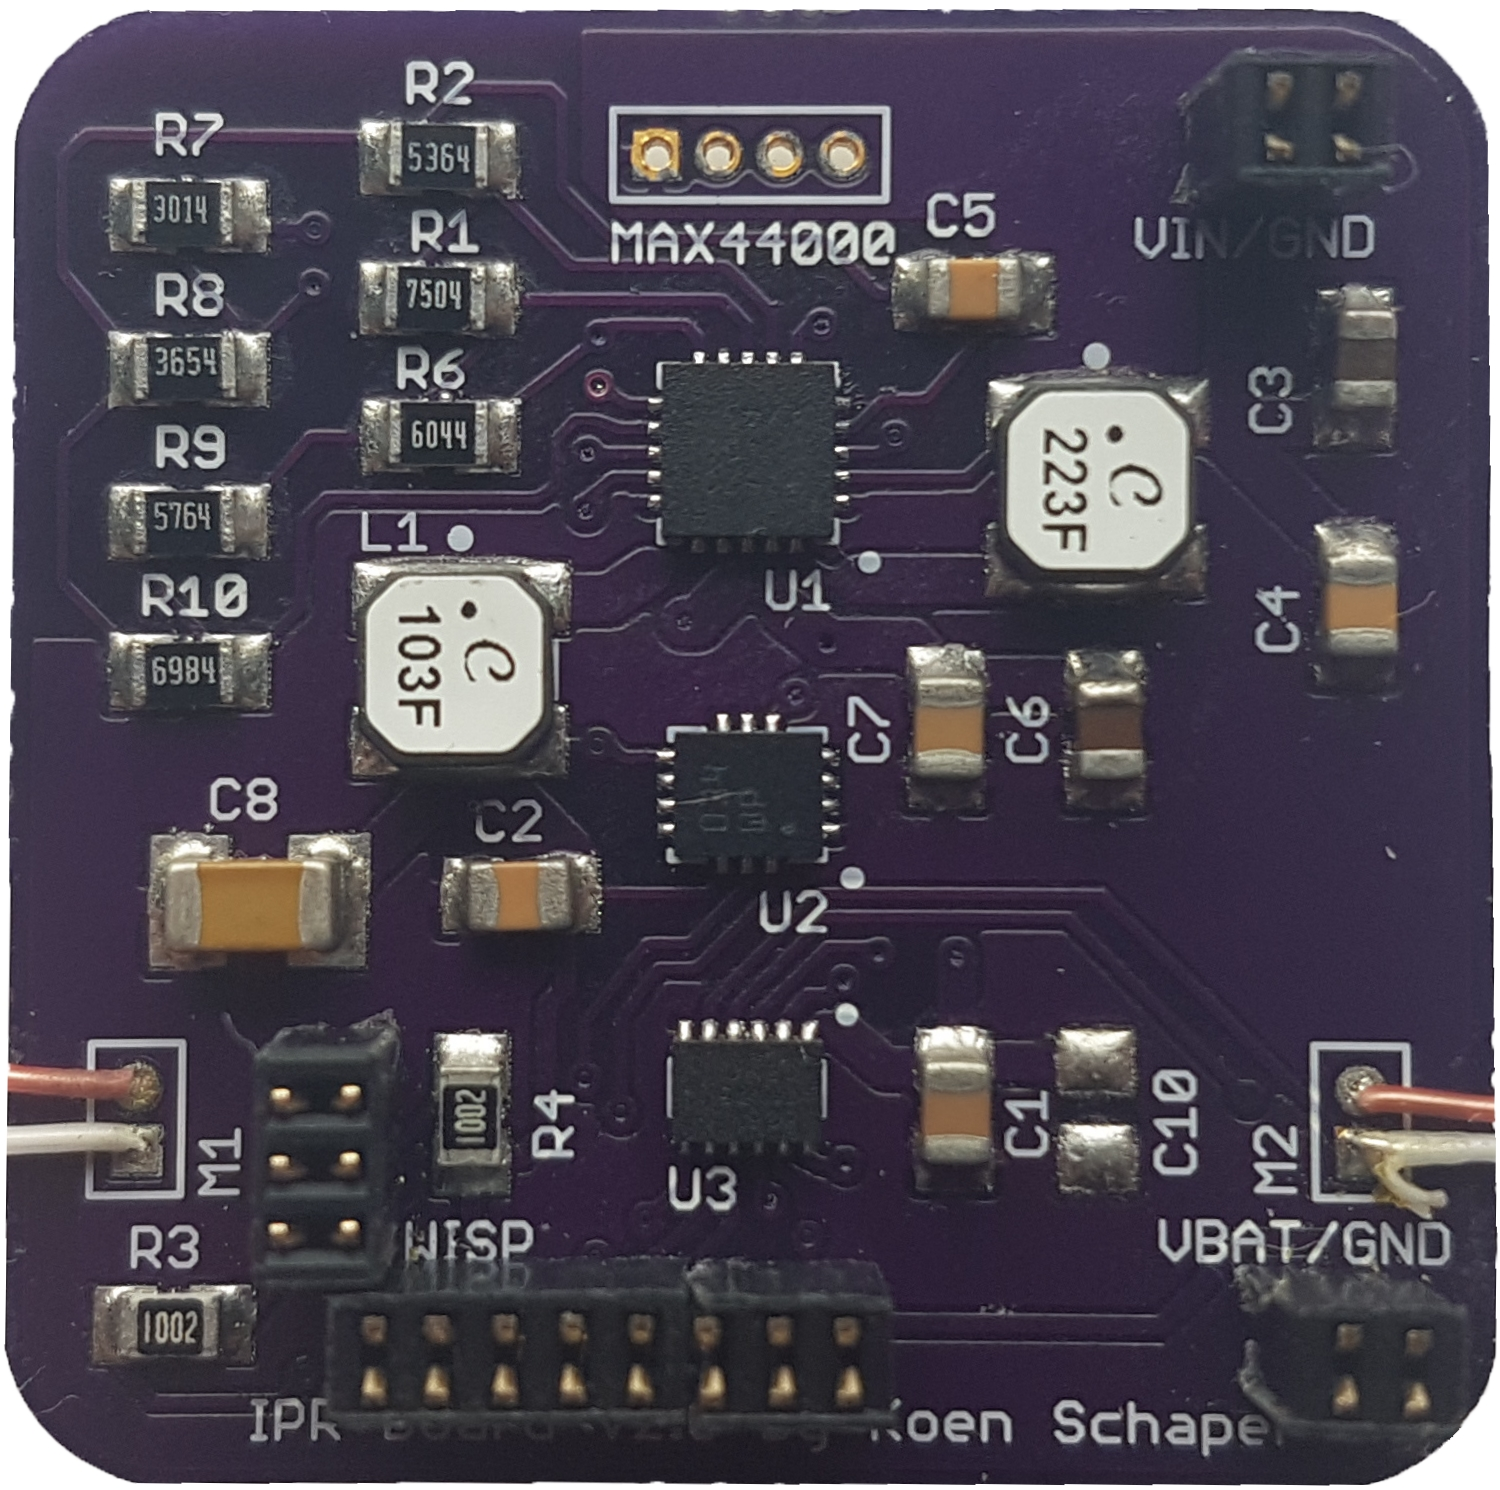
\includegraphics[width=\textwidth]{pics/pcb_front.jpg}
		\caption{Top side of the PCB}
		\label{fig:pcb_robot_front}
	\end{subfigure}
	\qquad
	\begin{subfigure}[b]{0.45\textwidth}
		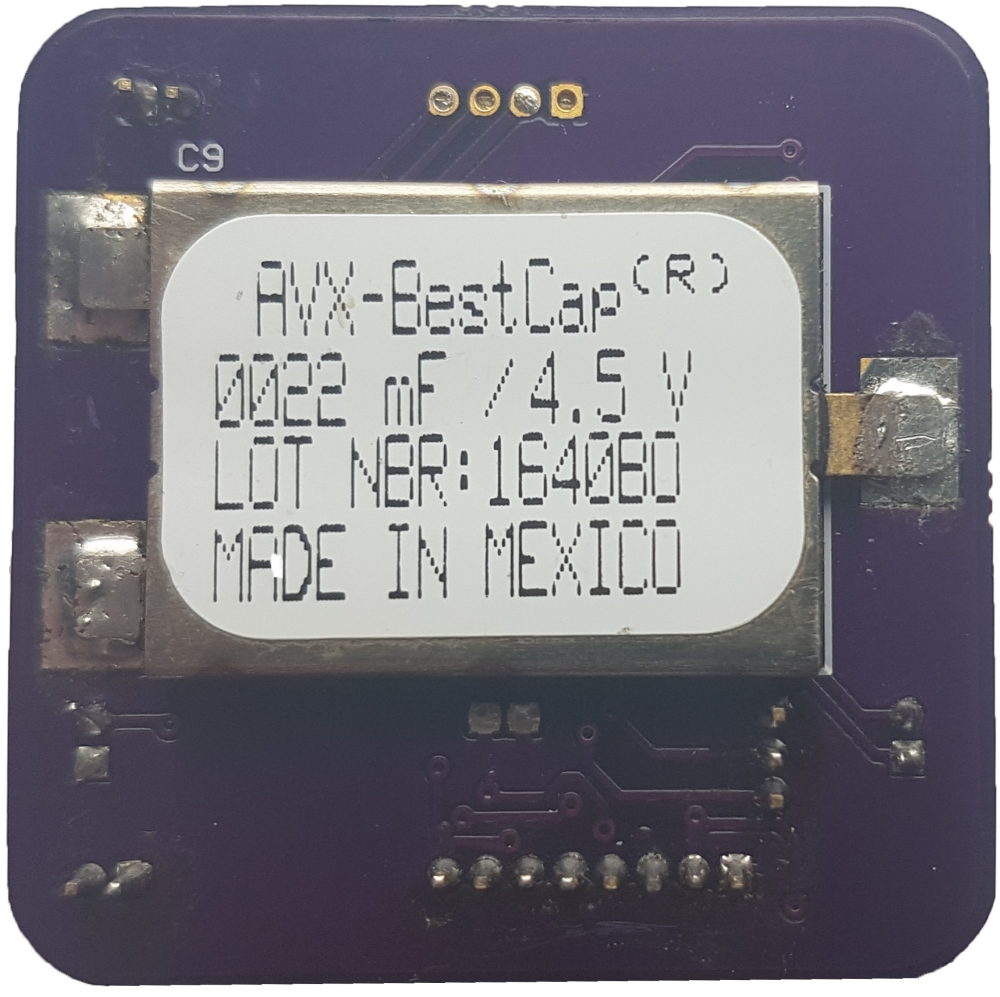
\includegraphics[width=\textwidth]{pics/pcb_back.jpg}
		\caption{Bottom side of the PCB}
		\label{fig:pcb_robot_back}
	\end{subfigure}
	\caption{The PCB designed for the robot}
	\label{fig:pcb_robot}
\end{figure}

\subsection{Energy Expenditure}

The average current consumed of each component was measured with a Monsoon Power Monitor~\cite{monsoon_powermonitor_2017}.
The measurement was preformed as follows, first a two second current trace was recorded of the current consumed by the MCU on the WISP.
The MCU was then used to enable each component individually, followed by a two second current measurement with the enabled component.
The average of each current trace was calculated, and the current consumed by the microcontroller subtracted from the current consumed by each component.
The measurement result is provided in Table \ref{tab:avg_cur_comp}.

% Make a overview of the cost to build a robot

\begin{table}[t]
	\centering
	\begin{threeparttable}
		\caption{Average consumed current for each individual component at 2.2 V.}
		\label{tab:avg_cur_comp}
		\begin{tabular}{|l|l|} 
			\hline
			Part & Active Current \\
			\hline\hline
			Proximity sensor & 119 \textmu A \\
			Gyroscope & 848 \textmu A\\	
			Microcontroller @ 8MHz & 522 \textmu A\\
			H-bridge & 349 \textmu A \\
			Two DC motors\textsuperscript{1} & 27--50 mA  \\
			\hline \hline
			Total & 29--52 mA \\
			\hline
		\end{tabular}
		\begin{tablenotes}
		\small
		\item [1] Current consumed varies per motor and motor speed
		\end{tablenotes}
	\end{threeparttable}
\end{table}

\subsection{Cost}

By using off-the-shelf components that that are readily available allows to build multiples of this robot with ease.
Keeping the cost down per individual is important when these robots are used in collectives.
Table \ref{tab:cost_robot} shows the total price to build a single robot, assuming a minimal fabrication quantity of 20.
This overview is compiled by querying the component prices of different suppliers, Farnell, Digikey, Mouser, Pololu, and OshPark.
The price for the PCB does not include the price of assembling the PCB, as this is currently done by hand.
Secondly, the cost of a WISP / MCU is currently not included in the price.
From this table can be concluded that the cost of building a transiently powered robot is comparable to the cost of other reference small robotic platforms.


\begin{table}[t]
	\centering
	\caption{Cost per robot}
	\label{tab:cost_robot}
	\begin{tabular}{|l|l|} 
		\hline
		Part & \euro Price \\
		\hline\hline
		Solar panel & 9,60\\
		Supercapacitor & 7,43\\
		Harvester & 5,48 \\
		Proximity sensor & 3,98 \\
		Gyroscope & 2,81\\	
		H-bridge & 1,47 \\
		Two DC motors & 18,51 \\
		Wheels & 3,08\\
		PCB & 2,50 \\
		Passive SMD & 4,53\\
		\hline \hline
		Total & 59,39 \\
		\hline
	\end{tabular}
\end{table}


\section{Control Design}

\subsection{Motor control}
\label{sec:calib_motors}

%TODO write intro and link to preliminaries
%When the motors are powered from the battery the supplied voltages drops while energy is consumed for the battery.
%Since the speed of the motor is dependent on the supply voltage the speed of the motor will also decrease while energy is consumed from the battery.
A benefit of keeping the supply voltage constant is that voltage is eliminated as a factor in determining the motor speed.
By making the assumption that the robot will only travel on a flat surface, the steady state speed is considered ``constant" given a certain PWM duty cycle.


\subsubsection{PWM Frequency for Linear Motion Control}
% Reference: https://www.precisionmicrodrives.com/application-notes/ab-022-pwm-frequency-for-linear-motion-control
%TODO update after writing preliminaries!

Pulse width modulation (PWM) is used to control the speed of the motors, the average current supplied to the motors can be regulated by changing the duty cycle.
When the motor is at rest its equivalent circuit consists of a resistance and inductance in series.
When voltage is applied to the motor the rate at which the current rises is limited by the inductance. 
All RL circuits have a time constant: $\tau = L / R$ and the current reaches its maximum steady state at $5\tau$. 
The motors used for the robot have a typical resistance R of 14.5\,$\Omega$ and an inductance of L = 70\,$\mu$H~\cite{gearmotor_206-110_2017}.
Therefore the minimum pulse width should be equal to

\begin{equation}
5\tau_{\min} = 5 \frac{L}{R} 
\end{equation}

From this can be calculated that the minimum pulse width should be $5\tau = 5 \cdot \frac{70 \cdot 10^{-6}}{14.5} = 24.14\,\mu s$.
If a minimum pulse width of is assumed, than the maximum PWM frequency becomes

\begin{equation}
f_{\max} = \frac{t_{\text{on}}}{5\tau}\cdot 100
\end{equation}

If the PWM frequency is assumed to be at least 5\% than the maximum PWM frequency is equal to $\frac{5}{24.14 \cdot 100} = 2071.25\,Hz$.
The PWM frequency will be set to 2\,kHz and later will be verified that the duty cycle will never go below the minimum of 5\%.

% -Write how the pwm control signals are generated for the H-bridge. 
The PWM signals are generated by the microcontroller on the WISP.
Four IO-ports are available on the WISP which can be directly controlled by a single timer.
The timer is configured to use a compare register for each of the ports.
When the timer reaches a value that corresponds to a value one of the compare registers the connected port is toggled automatically.
This way the overhead is minimized because no interrupt service routine is required.

\subsubsection{Minimal Duty Cycle}

The minimal PWM duty cycle to produce a torque that is able to overcome the static friction between the wheels and a surface the robot is moving on.
Each motor is physically different and the friction in the gearbox can variate as well, which results in a variating output speeds per motor.
Since the robot uses two motors in differential drive configuration, a minimum PWM duty cycle has to be found for each motor.
This is accomplished by setting a PWM duty cycle at which both motors are rotating and slowly backing down the PWM duty cycle until one or both stop turning.
The minimum PWM duty cycle, allowing the wheels to rotate, is stored as a calibration and added to every motor set point.
If the robot is set to run at the minimum speed does not mean that the motors run at the same speed.


\subsubsection{Maximal Duty Cycle}
% -Write about maximum speed due to enabling two motors and their startup current peak! show figure!!
% Does more gearing (more torque) reduce the current peak??

The maximum PWM duty cycle is bounded by the amount of current that the buck converter and bulk capacitor can supply.
In Section \ref{sec:pre_dc_motor_locomotion} the current profile of a DC motor is determined by modeling the DC motor with its corresponding parameters.
Lowering the PWM duty cycle reduces both the maximum current peak and the steady state current and therefore can be used to reduce the motor start current demand.
The maximum PWM duty cycle can be found by increasing the duty cycle until the robot is not able to start a movement from that PWM set point.


\subsection{Closed loop feedback for controlled movements}

%The robot uses two physically different motors in differential drive configuration which are mounted in a non-symmetrical way.
Open loop movement using just a calibrated motor values has been used in previous work \cite{legoc_uist_2016}, but it can be time consuming and any little disturbance will trow the robot off course.
Controlled movements are possible using closed loop feedback, where the heading is used to update the motor control values.
The robots change in heading can be obtained from the gyroscope and corresponds to the yaw-rate.

\subsubsection{PID Controller}

% -Why pid for straight movements and not a simple p controller?
% --Fast reaction on disturbances without osccilation??
%TODO -Write about bounding the pid output, because otherwise the motors of the robot could stall, if the motor setpoint is to high

Closed loop feedback is achieved by use of a Proportional Integral Derivative (PID) controller.
The input of the PID controller is the yaw-rate from the gyroscope.
The controller will periodically try to reduce the yaw error as follows

\begin{equation}
	e(t) = \psi_{\text{target}} - \psi(t)
\end{equation}

\noindent
where $\psi_{\text{target}}$ is the yaw-rate target and $\psi(t)$ the yaw-rate obtained by the gyroscope.
The PID controller will now adjust its output and correct the speed of each motor, in opposite direction, by the following equation

\begin{equation}
u(t) = K_{p}e(t) + K_{i} \int_{0}^{t}e(\tau)d\tau + Kd\frac{d}{dt}e(t)
\end{equation}

\noindent
where $K_{p}$, $K_{i}$ and $K_{d}$ are the tunable gains from the PID controller.

\subsubsection{Controlled straight movements}

For controlled straight movements horizontal movement is undesired, therefore the target yaw-rate is set to zero.
The controller will continuously adjust the motor speed in order to achieve this.

\subsubsection{Controlled curved movements} 

Instead of an angular velocity set point of zero, an turn rate needs to be specified.
This desired angular velocity can be a determined from the radius of the circle that the robot needs to turn and the calibrated target speed.

\subsubsection{PID tuning using Ziegler-Nichols method}

%TODO -Write about tuning the pid controller using Ziegler–Nichols tuning method (method 2), closed loop, Critical gain.

Tuning can be done by a trail and error approach but a faster way of tuning is to use the Zigeler-Nicholos method.
It starts with increasing or decreasing $K_{p}$ until constant oscillation occurs.
From Figure \ref{fig:ultimate_gain} can be seen how the proportional gain was increased until eventually the robot started to oscillate.
With a proportional gain of 0.13 the robot starts light oscillation at the end, but this is not always the case and can be a result of the surface the robot was driving on.
% Tell something about how the right values are determined
To reduce the oscillation a $T_{u}$ of 0.2 was added as can be determined from Figure \ref{fig:gain_tuning}.
From this figure can be seen that the robot is more stable and does not have the tendency to oscillate anymore.
%Robots was driving on surface that was not super flat, therefore the gyro signal is noisy.
The tuning process was speeded up by setting the minimum motor duty cycle as it made the robot a lot more responsive, this was described earlier in Section \ref{sec:calib_motors}.

%TODO -Add figure with critcial gain + mark period Tu

\begin{figure}
	\begin{subfigure}[b]{0.49\textwidth}
		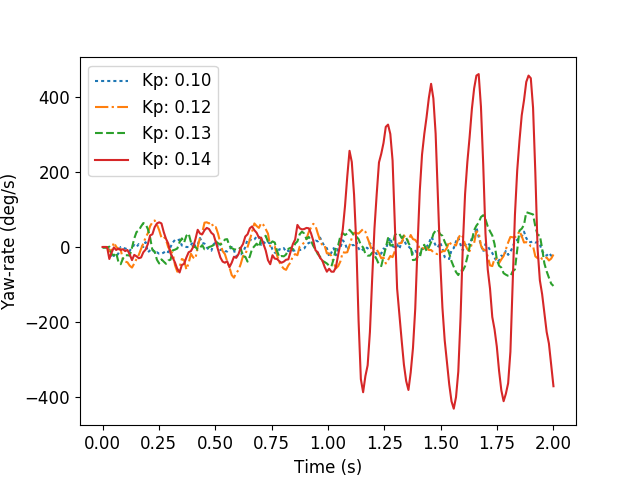
\includegraphics[width=\textwidth]{pics/straight_ku.png}
		\caption{Increase $K_p$ until constant oscillation}
		\label{fig:ultimate_gain}
	\end{subfigure}
	\begin{subfigure}[b]{0.49\textwidth}
		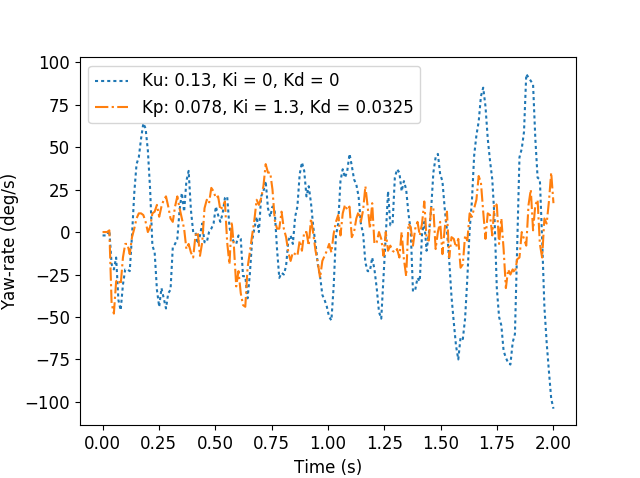
\includegraphics[width=\textwidth]{pics/straight_ku_with_tu.png}
		\caption{Find the constant oscillation period}
		\label{fig:gain_tuning}
	\end{subfigure}
	\caption{Tuning the PID controller using the ultimate gain method.}
\end{figure}

\subsubsection{Controlled turns}

The control loop for controlled turning uses the angle, which is obtained by integrating the yaw-rate sensor data from the gyroscope.
A P controller is used to rotate the robot to the desired angle, the proportional gain is directly influencing turn speed of the robot.
The motor control values are set to run the motors opposite directions and are equal to the output of the P controller.
These values will keep decreasing until the robot rotates to the desired angle.
The set point is assumed to be reached when the angle is within two degrees of the target, in this case the loop will stop automatically.
To allow enough precision to measure if the target is within these two degrees, the timer which executes the control loop was set to run at 100\,Hz.
Secondly, the proportional gain should not be set to low because the robot might not able to reach the target but also not to high as it can overshoot the target.

\section{Software Implementation}

The robot can be controlled using three different commands, one for straight trajectories, one for left and one for right turns.
When a command is executed a control loop will run until the provided target is reached.
A timer running periodically calling an interrupt service routine which executes the control loop.   
Each command requires different initial values, set points and tuning parameters, these are set accordingly before the control loop is enabled.

\subsection{Controlled straight movements}

Target motor speed 
Using the output of the PID controller the target motor speed of each motor is adjusted in opposite direction.

The loop will stop automatically when the required target is reached.
%TODO Explain that the target distance is with a calibrated value.

\subsection{Controlled curved movements}
The same PID control loop can be used to command the robot to make curved movements.
By integrating the angular velocity an angle estimate is obtained, which is used to verify if the angle target given is reached within two degrees.
In case this is true the loop will exit automatically.


\subsection{Persistent movement}

Normally when a robot is battery powered, it can execute some predefined movements and stop when required.
In case of the transiently powered robot one movement or a series of movements is likely to require multiple power cycles to complete.
To be able to finish a movement and not reset i.e. redo the same movement, a simple check pointing method is used to keep the program state across power cycles.
A persistent counter registers the progress in the set of movements.
In the control loop only the progress in moving towards a set point is stored in non-volatile FRAM memory, which depending on the movement can be a required time or angle.
The right and left motor speed which are tuned by the controllers are not saved and restored after a power interrupt.
The motors have a startup phase the controller needs to react differently compared to the steady state, constant speed movement of the robot. 

\chapter{Evaluation} 

% - Weight vs current consumption vs distance
% - Measure start motor overhead and average consumption (show graph?)


\section{Performance in different light conditions}
% Casestudy of conditions robot 
% outdoors/indoors/varying light sources/varying solar panels
% Do experiment in sunlight for nuna panel

%The amount of energy that can be harvested from normal office lighting is limited.
Currently the robot harvests energy form light using a small solar panel.
However, there isn't always enough sunlight available to charge the robots in a acceptable time.
To allow the robots to have sub ten second charge times, a lighting setup needs to be created that provides a reasonable amount of uniform light to the area where the robots move around.
In this section the charge time of the supercapacitor is evaluated, while it's charged from different solar panels and different light sources.

\subsection{Experimental setup}
% Temperature and Light intensity?
To accurately measure the power that is harvested from each solar panel all the experiments were preformed in a darkroom.
The setup consists of a light source that can be positioned at multiple distances from a solar panel.
The solar panel is connected to input of the harvester on the PCB of the robot and when the voltage in the supercapacitor reaches the threshold the buck converter of the energy harvester is enabled.
Voltage is supplied to the WISP which is programed to only enable a GPIO port and enable a LED.
A Saleae Logic, logic analyzer is connected to the port and used to record the time required to charge the capacitor from the minimum to the maximum value.
The port is enabled the light source is disabled and the LED is used to drain the energy from the capacitor.
When the led turns off, indicating that a new charge period begins, the light source is enabled again.
Now a more detailed description will be given of the different components that were tested.

%TODO Why these lamps?
Three different solar panels were tested in this experiment. Information about the solar panels can be found in Table \ref{tab:solar_panels}.
Low cost solar simulators can consist of a combination of LED and halogen light bulbs to simulate sunlight and are used to test the performance of solar panels~\cite{grandi_tia_2014}.
However, in this case the goal is to have a controlled uniform lighting environment where the robots have roughly constant charge times.
Solar panels do not only harvest energy from the visual light spectrum but harvest almost at least as much from the infrared light spectrum, therefore not only light but also heat will shorten the charge time.
Halogen lamps have a lower color temperature than the sun but also emit waves far into the infrared spectrum.
The light sources used in this experiment are a 60W halogen bulb, a 120W halogen halogen bulb and two 150w IR heat lamps where one is colored red.
Three measurements were done, where the lamps were positioned 10cm, 30cm and 50cm from the solar panels.
Additionally, for these three distance the temperature was measured at the solar panel using a K-type thermocouple supplied with an Extech EX330 multimeter and the light intensity using the luxmeter on a MASTECH MS8229 multimeter.

\begin{table}[t]
	\centering
	\begin{threeparttable}
		\caption{The solar panels tested in the experiment}
		\label{tab:solar_panels}
		\small
		\begin{tabular}{|l|l|l|l|}
			\hline
			& Composition & Efficiency & Dimensions \\
			\hline \hline
			Banggood \cite{bangood_solar_2017}& Poly-Si & 17\% & 40x30mm \\
			\hline
			INYS SLMD121H04L-ND\textsuperscript{1}& Mono-Si & 22\% & 43x34mm \\
			\hline
			Azurspace 3G28C & Triple Junction GaAs& 28\% & 80x40mm \\
			\hline
		\end{tabular}
	\begin{tablenotes}
		\small
		\item [1] Two panels in parallel
	\end{tablenotes}
	\end{threeparttable}
\end{table}

\subsection{Results}
% No difference between the heatlamps in power consumed
% Halogen distributes the light more even
% Panel from nuna
% Refer to appendix for temperature and light data?

Both the temperature and illumination increase by decreasing the distance between the light source and the solar panel. 
Secondly, increasing the output power of the lamp increases temperature and illumination as well. 
However the charge times 
A thing to note is that the both the 60w and 150w ir lamps have a spherical design. This creates a uneven circular shadowing pattern on the surface the lamps are shining on, which becomes more significant on the bigger distances in this experiment.
The 120w lamp has a tubular design and in combination with the light fixture most of the light is reflected down with minimal shadowing of the lamp resulting in a more even light distribution.

\begin{figure}
	\centering
	\begin{subfigure}[b]{0.49\textwidth}
		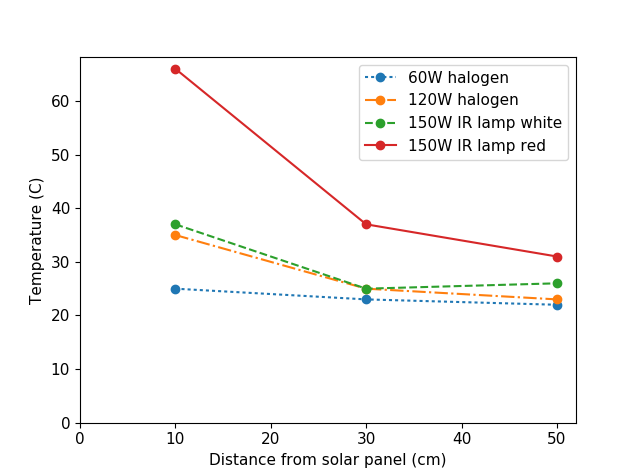
\includegraphics[width=\textwidth]{pics/light_experiment_temp.png}
		\caption{Temperature at different distances}
		\label{fig:light_temp}
	\end{subfigure}
	\begin{subfigure}[b]{0.49\textwidth}
		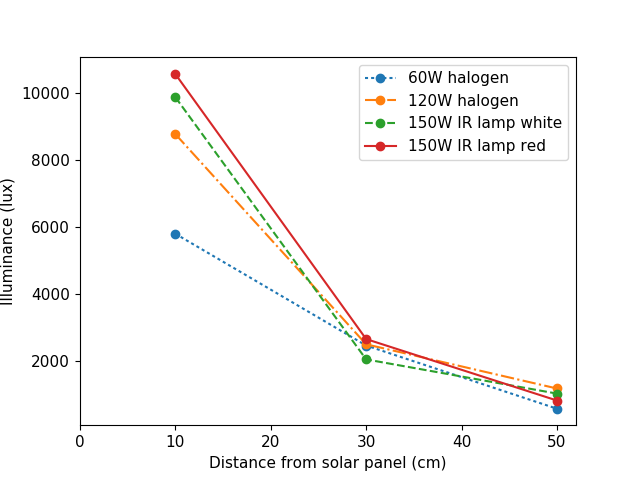
\includegraphics[width=\textwidth]{pics/light_experiment_lux.png}
		\caption{Light intensity at different distances}
		\label{fig:light_lux}
	\end{subfigure}
	\caption{}
\end{figure}


\begin{figure}
	\centering
	\begin{subfigure}[b]{0.49\textwidth}
		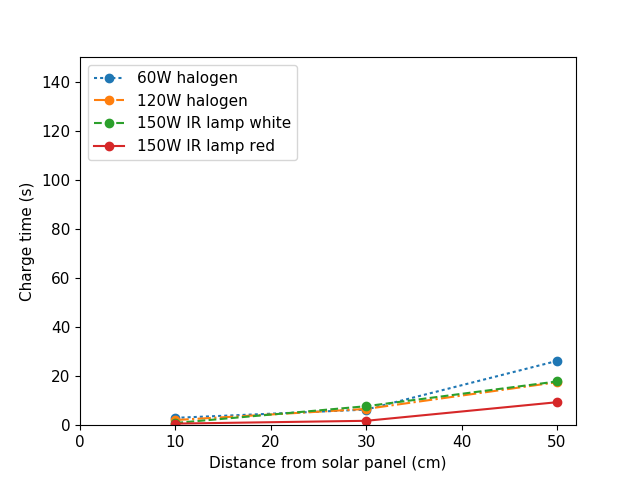
\includegraphics[width=\textwidth]{pics/light_experiment_figure1.png}
		\caption{Ebay panel}
		\label{fig:light_exp1}
	\end{subfigure}
	\begin{subfigure}[b]{0.49\textwidth}
		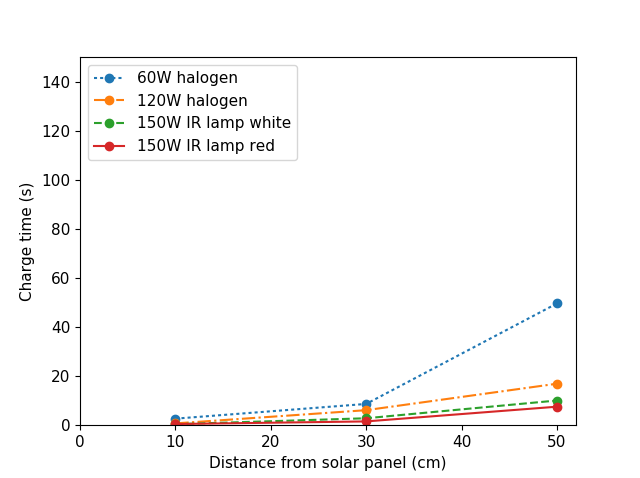
\includegraphics[width=\textwidth]{pics/light_experiment_figure2.png}
		\caption{IXYS SLMD121H04L-ND}
		\label{fig:light_exp2}
	\end{subfigure}
	\begin{subfigure}[b]{0.49\textwidth}
		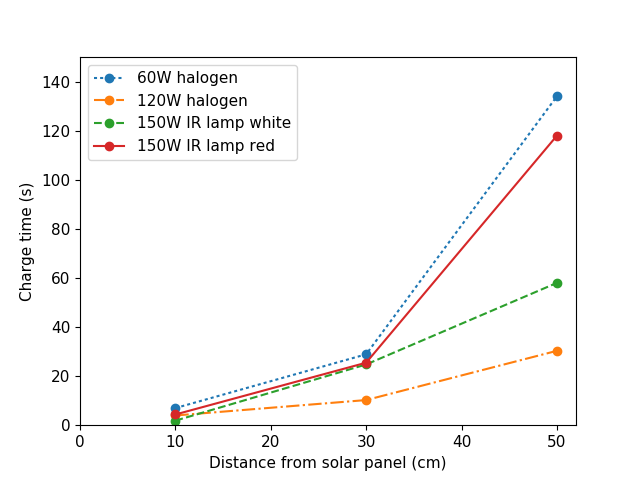
\includegraphics[width=\textwidth]{pics/light_experiment_figure3.png}
		\caption{Azurspace 3G28C}
		\label{fig:light_exp3}
	\end{subfigure}
	\caption{The performance of three different solar panels for different distances from different light sources. The data charge times for the last two are normalized with respect to the surface covered by the first panel.}
\end{figure}


\section{Controlled Movements}
\label{sec:controlled_movements}

% Comparison deadreckoning accuracy of battery powered robot with solar powered robot

% Try at least one more supercapacitor: 10mF
% Study reducing the frequency of power interrupts ie smaller energy buffer.
% How does this effect the accuracy of locomotion?

% Study the effect of checkpoint frequency on the straight and turn accuracy + combination
% Before and after counting in case of current robot

% Video of robot movement

Now that a variety of solar panel / light combinations has been evaluated, the next Section will evaluate the accuracy of movement of the robot and will compare the battery-less robot and it' battery powered equal.

\subsection{Experimental setup}

To be able to compare the accuracy of the robot while it is exposed to increasingly smaller power cycles, a variety of movements is recorded using a overhead camera.
A camera stand with DSLR camera is positioned on a tabletop and in the camera's view the corners of a square of 80 x 80 cm are indicated with a black marker, see Figure \ref{fig:movement_setup}.
This square can later be used as a reference to convert the robots movement from pixels to cm.

Three different movements are compared, while the robot is moving straight movement of 75 cm, a circle with radius of 30cm and a square of 50 by 50 cm.

\subsubsection{Artificial Power Interrupts}

%TODO Why bat powered
During the experiment the robot will be powered from a battery and power interrupts, i.e the capacitor running out of energy are created artificially using a timer that resets the MCU.
The MSP430FR5969 has the functionality to enable a brownout reset trough software which is used to simulate the event of the supply voltage dropping below the required operating voltage.
With a capacitor of 22mF the robot can operate around 1 second, this resulted in the chosen interrupt periods.
Choosing a period smaller than half a second resulted in uncontrolled behavior, while the control loop was not able to stabilize the movement before the robot runs out of energy again.
Therefore the power interrupt periods evaluated in this experiment are: 1.25, 1, 0.75 and 0.5 seconds.

\subsubsection{Velocity calibration}

%TODO make table with standard deviation of distance traveled 
Each movement is executed at three different PWM target settings: 40\%, 65\% and 90\% of the maximum duty cycle.
To let the robot move a particular distance, the average speed needs to be estimated for each PWM target and power interrupt period.
This is achieved by first determining the time that the robot requires to move approximately 150 cm for each target without power interrupts.
When the robot experiences power interrupts the average velocity of a active period becomes lower due to frequent acceleration from standstill.
With power interrupts the runtime is increased to make the robot travel roughly the same distance.
Finally, the average of five measurements is computed and divided by the commanded runtime of the robot to acquire an average speed for each combination.


\subsubsection{Tracking the robots Movement}

A robot is programmed to preform the movement at a desired velocity and optional power interrupt period.
Before the robot executes the movement a green led is enabled on top of the robot, this bright green dot will be the reference point that the tracking software will try to follow.
The camera is used to record the movement which is analyzed using Python and OpenCV 3.2, a example of a tracked movement can be seen in Figure \ref{fig:movement_example}.

\begin{figure}
	\centering
	\begin{subfigure}[b]{0.45\textwidth}
		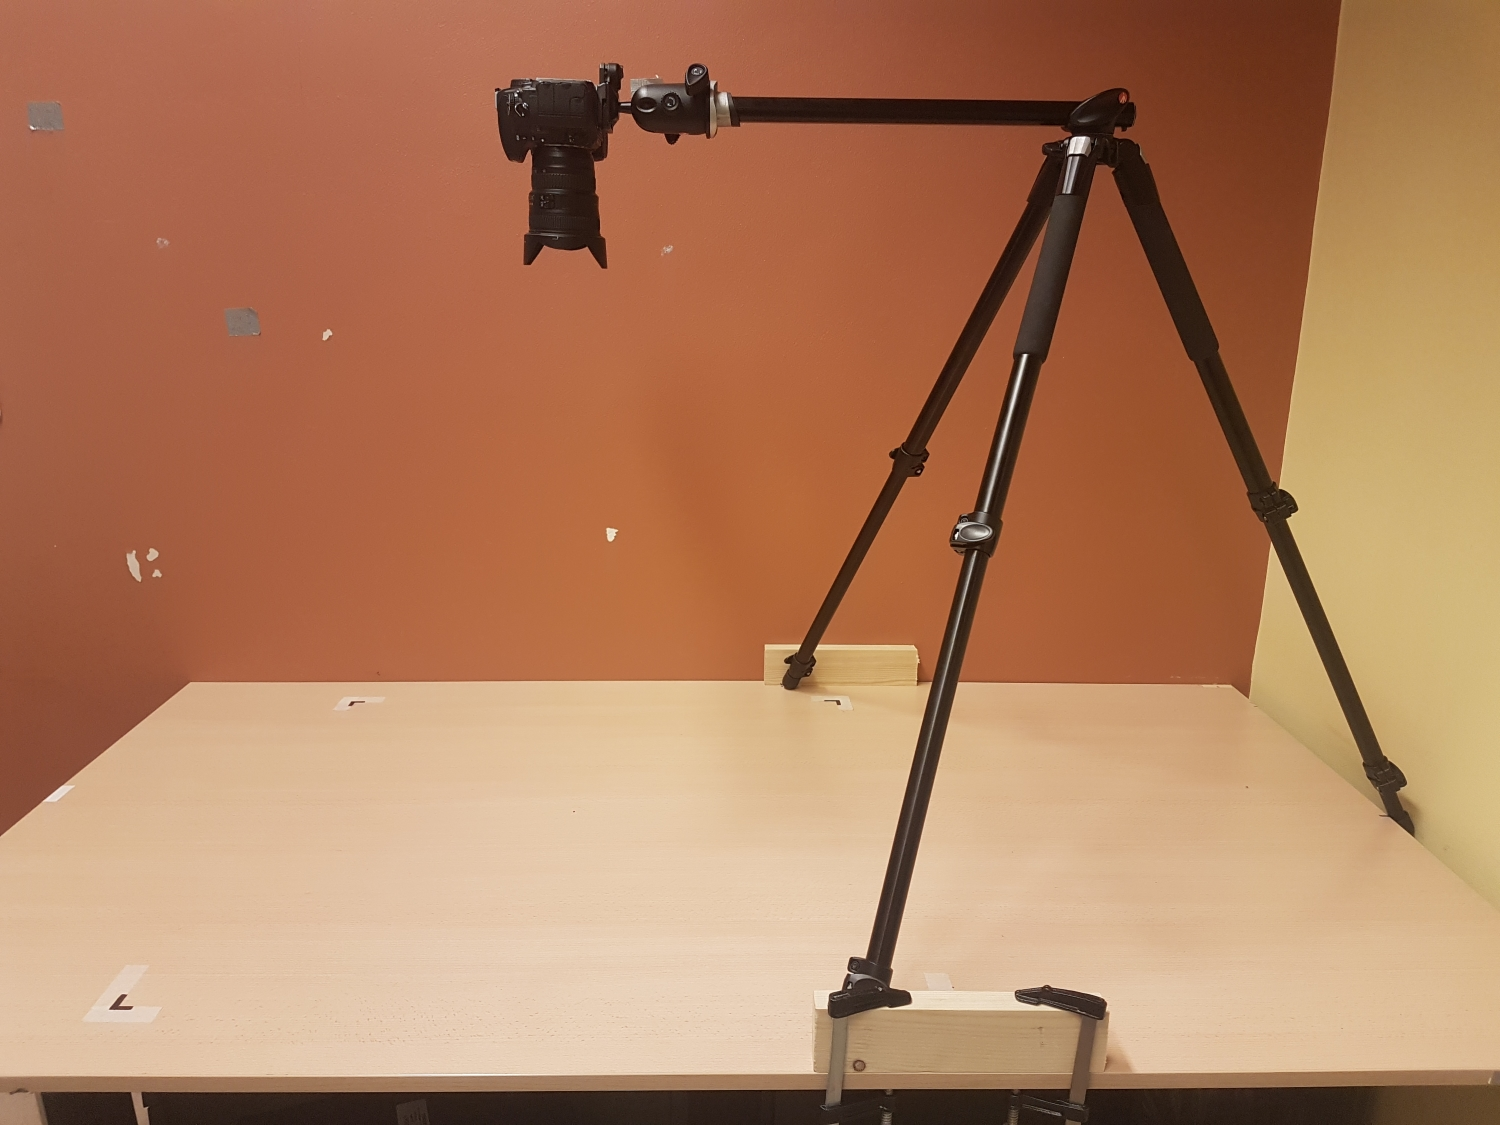
\includegraphics[width=\textwidth]{pics/movement_setup.jpg}
		\caption{Camera setup}
		\label{fig:movement_setup}
	\end{subfigure}
	\quad
	\begin{subfigure}[b]{0.45\textwidth}
		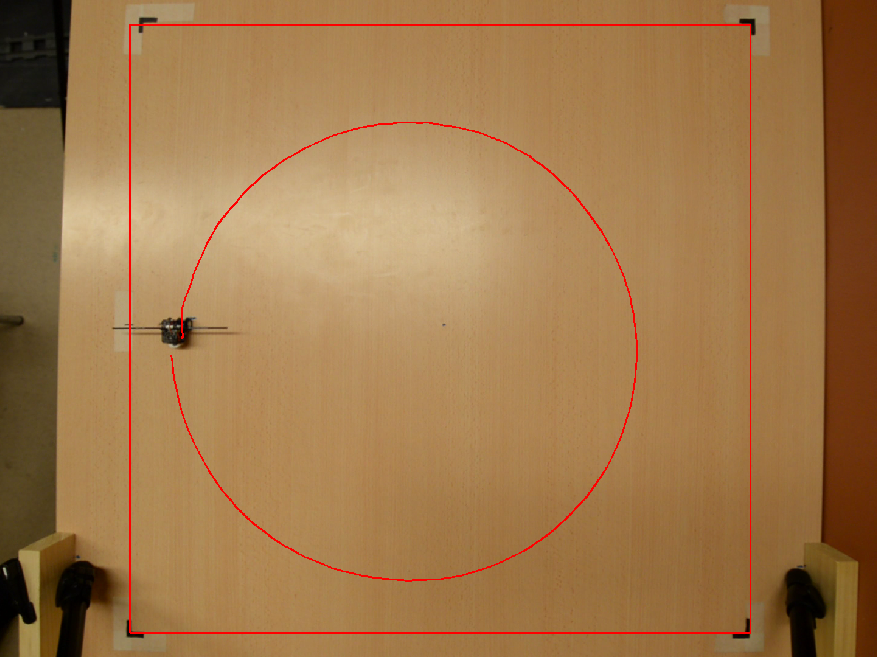
\includegraphics[width=\textwidth]{pics/movement_example.png}
		\caption{Tracking with OpenCV}
		\label{fig:movement_example}
	\end{subfigure}
	\caption{Recording the robots movement}
\end{figure}


\subsection{Movement Accuracy Metrics}

for straight movements: the amount of curvature

standard deviation in length of movement for each type of movement

\subsection{Straight Movements}




\subsection{Curved Movements and Turns}


\subsection{Results}

Hoe de interrupts uitkomen op de beweging heeft invloed!!

Lager snelheid en minder interrupts is hogere precisie??




% CONCLUSIONS AND FUTURE WORK
\chapter{Summary}
\label{chp:summary}

%This thesis is surmised by a conclusion in Section \ref{sec:conclusion} and in Section \ref{sec:limitations_future_work} possibilities for future work will be presented.

\section{Conclusion}
\label{sec:conclusion}

In this thesis, a transiently-powered robot is designed and implemented that uses light as a source of energy.
Two geared dc motors have been chosen to provide locomotion to the robot and their startup current peak is limited using PWM.
A controller is designed that allows for controlled straight and curved movements, while a simple check pointing method combined with persistent movement targets allows a movement to be completed across multiple power cycles.
Multiple movements have been executed and recorded using an overhead camera.
Tracking software is used to verify the accuracy of a transiently-powered battery-free robot and compares it performance to a battery powered equivalent robot.
By decreasing the interrupt period, a lower threshold of 0.3\,s has been found in which case the robot started to show uncontrolled behavior, i.e. significant drift to the side of the weakest motor.
The amount of time that power is available might not be sufficient for the motors to reach their steady state speed, making controlled movements using linear motor control impossible.
Using artificial power interrupts, the results show that decreasing the interrupt period towards the lower threshold results in increased horizontal deviation in case of straight movements.
This is suspected to be caused by more frequent accelerations from standstill.
For curved movements the results show a decreased average deviation from the fitted circle by increasing the target duty cycle.
The additional speed is suspected to allow the controller to be more effective in steering the robot towards its final destination.
The solar powered robot surprisingly outperforms the battery-powered robot in terms of movement accuracy, as the additional weight of the solar panel is suspected to have a positive effect on the movement of the robot.

%Section \ref{sec:controlled_movements} shows that the transiently powered robot is able to execute an instructed motion with similar accuracy compared to a battery powered equal. 
%The distance covered by a robot with frequent power interrupts in a certain amount of time is smaller, i.e the average speed is lower due to frequent acceleration from a standstill.

\section{Future Work}
\label{sec:limitations_future_work}

The capabilities of the current robot can easily be extended by using more features from the WISP or by designing a custom alternative.
Additional features that could be implemented in future work are:

\begin{itemize}

\item \textbf{Speed feedback}: 
In order to move a certain distance with a higher accuracy, an energy efficient speed feedback method is required.
One option is to add local speed sensing or another option is to supply external position feedback to the robot.

%One option could be to determine motor speed by measuring the Back-EMF produced by the motor, as it is proportional to the motors revolutions per minute~\cite{precision_backemf_2017}.
%Another method could use wheel encoders without an active light source and instead use ambient light, already available in abundance because it is used as the source of energy.

\item \textbf{Lack of communication}: 
Communication with an external host is not implemented.
The energy efficient backscatter communication channel of the WISP could be used.
Even though power cycles will occur less frequent when compared to the RFID, due to relative large supercapacitor, they still pose a challenge in externally controlling the robot.

\item \textbf{Transiently-powered swarm}: 
With a communication channel, a new promising area of research is to create a swarm of transiently powered robots.
The effect of intermittentcy on the behavior and controllability of this type of swarm needs to be investigated.
This research could further investigate the portability of existing swarm algorithms or propose new solutions.	

\item \textbf{Size reduction}: 
In order to further reduce the weight of a robot there is a need to move away from DC-motors, since significant smaller and efficient DC-motors are not available.
%Alternative legged locomotion types have been discussed in Section \ref{sec:rw_locomotion}.
Miniature legged robots that make use of piezoelectric actuators seem promising, but most of them are still in an early stage of development.

\item \textbf{Sensing capabilities}: 
Future applications may require additional sensors to be added to the robot to extend its capabilities.
However, the power consumption, frequency of use and the accuracy trade off needs to be evaluated carefully since the energy budget is limited.


\end{itemize}

%\item \textbf{TP swarm OS} 
%Recently, embedded operating systems~\cite{trenkwalder_iros_2016} and extendable programming~\cite{pinciroli_iros_2016} languages have been created to speed up the development process of swarms, removing the need to focus on low level interactions and individual behaviors.
%In addition, multiple task and checkpoint based methods have been developed to enable computation across power cycles as described in Section \ref{sec:comp_pc}.
%Merging both paradigms could help to speed up development of transiently powered swarms. 



%\subsection{Path planning based on energy availability}

%To capture the optimal amount of solar energy along the way, a map of the expected solar power can be used to compute the optimal path. To distinguish sunny or shaded two methods are proposed in \cite{plonski_tranro_2016}, one being a simple data driven Gaussian Process and the other estimates the geometry of the environment as a latent variable.
%Energy aware path planning is commonly used in combination with mission planning.
%In \cite{kaplan_iros_2016}, an analysis of the solar radiation is used to generate a time-optimized motion plan and power schedule using a cascaded particle swarm optimization algorithm.
%By combining maps of lighting and ground slope a solar-powered robot can be kept illuminated continuously. A connected component analysis is used to plan a optimal route on traversable slopes, as described by \cite{otten_icra_2015}.

% BIBLIOGRAPHY
%#define SORTED 1
%\bibliographystyle{../bib/latex8}
%\bibliography{../bib/bibtex}

\bibliographystyle{IEEEtran}
\bibliography{IEEEabrv,bib/bibtex,bib/non-paper}

\appendix
\chapter{TODO APPENDIX NAME}
\label{app:}
Appendix body



\end{document}

